\documentclass[12pt]{article}
\usepackage[paperwidth=8.5in,paperheight=11in,margin=1in]{geometry}
\usepackage{float}
\usepackage{lipsum}
\usepackage{parskip}
\usepackage{bbding}
\usepackage{amssymb}
\usepackage{titlesec} 
\usepackage{graphicx}
\usepackage{hyperref}
\usepackage{setspace}
\usepackage[normalem]{ulem}
\usepackage[section]{placeins}
\usepackage[toc,page]{appendix}
\newcounter{subsubsubsection}[subsubsection]
\newcommand{\tline}{\hspace{-2.3pt}$\bullet$ \hspace{5pt}}
\hypersetup{colorlinks=true, linkcolor=black, urlcolor=blue}
\setlength{\parindent}{15pt} % Indent paragraphs (automatically)
\usepackage{pdfpages, caption}


\makeatother
\makeatletter
\setlength{\@fptop}{0pt}

\newcommand\tab[1][1cm]{\hspace*{#1}}

\definecolor{myRed}{RGB}{248, 0, 0}
\definecolor{myGreen}{RGB}{0, 208, 0} %full green too light -P
\definecolor{myBlue}{RGB}{0, 0, 248}

\begin{document}
	\begin{titlepage}
		\centering	
%		\vspace{.25cm}
    
    \begin{figure}[h]
      \centering
%      \includegraphics[width=0.45\linewidth]{icon for team goes here}
    \end{figure} 
  
  {\huge\bfseries \textcolor{myRed}{L}\textcolor{myGreen}{E}a\textcolor{myBlue}{D} Design: \\ Design Report\par}
    
    \title{}
    \date{\vspace{-5ex}} %blank date -P
    \author{%
    	\makebox[.3\linewidth]{\Large\itshape Adrian Beehner}\\Budget Director\\beeh9036@vandals.uidaho.edu
    	\and \makebox[.3\linewidth]{\Large\itshape Andrew Butler}\\Documenter\\butl6046@vandals.uidaho.edu
    	\and \\ \makebox[.3\linewidth]{\Large\itshape Kevin Dorscher}\\Client Liaison\\dors7905@vandals.uidaho.edu
    	\and \\ \makebox[.3\linewidth]{\Large\itshape Paul Martin}\\Designer\\mart2659@vandals.uidaho.edu
    }
    \let\newpage\relax\maketitle %don't make a new page -P
    \maketitle		
    
    \vspace{4cm} 
    
    {\scshape\Large 
      CS 480/481: Fall 2017 - Spring 2018 \\
      Senior Capstone Design Project \\ 
      UI CS - Wireless Tower of Lights \\
      Sponsor - Dr. Robert Rinker
      \par}
    
     \vspace{3cm} 
    
    \begin{figure}[h]
      \centering
      
\includegraphics[width=0.7\linewidth]{assets/uislogan.png}
    \end{figure} 
  
		\vfill		
	\end{titlepage}

	\tableofcontents
	\newpage
	
	
		\section{Executive Summary}
		The University of Idaho has a Tower of Lights Show. The current "TowerLights" product involves LED-based light bars that are placed in front of front-facing widows of a large buildling (Theophilus Tower) and are then illuminated to play animations alongside/synchronously with music, the design is turning the project into a wireless system.\\
		The goal is to enhance the current "TowerLights" product, To convert the system to a wireless operation. This requires the development of a wireless module that would be attached to each of the light bars. Thus this module has to sleep and wake up, as well as respond to wireless signals from a computer, these modules will need to be battery powered. Battery power must also be conserved by staying in the sleep state until needed. The purpose of this enhancement is to provide a certain level of portability. The features and solutions of the product are utilzing a 9V Li-Ion Battery with 600 mAh for power, also using the 802.15.4 (Zigbee) protocol with channels of 3 btyes. The product uses low power mode offered by the Atmega 328P microporcessor. Reviever modules on each lightbar (Zigbee) are featured as well. Finally, utilizing Zigbee protocol, to avoid Wifi interference. The product gives the user the ability to run a program that reads in .tan files and .wav files, have this program communicate with a XBee Wireless module on an Arduino that is attached to a computer via USB, then communicate wirelessly with the Arduino receivers. Each of these Arduino receivers are attached to an LED board, that will then communicate with each LED on that board through wired communication from the Arduino to the LEDs. The program that broadcasts the shows will be available for Linux based operating systems.\\
		The merits of this system are in technical aspects the abiltiy to have a mobile light show system. This allows almost any building configuration to host a light show. Low-power mode allows easy setups for shows. In terms of business, the mobility allows other interested parties besides the University of Idaho to utilize this technology.\\
		The test results conducted focus primarily on the bettery. Operation time is around two hours, and has been tested on mutliple accounts, on muitlple light bars. Other test reults include brightness of LEDs, and low-power mode, whose results came back to suggest use of 4 LEDs, and a low-power mode waking up every minute and a half. 
		
		\newpage
	
		\section{Background}
		The University of Idaho has, for several years, done various projects involving the Tower of Lights Show and equipping the marching band with light-up glasses. The current "TowerLights" product involves LED-based light bars that are placed in front of front-facing widows of a large buildling (Theophilus Tower) and are then illuminated to play animations alongside/synchronously with music. The goal is to enhance the current "TowerLights" product. The current implementation of this product uses the ethernet wiring system in the building to control the LEDs. The goal of the project described is to convert this part of the system to a wireless operation. The motivation of this enhancement is to provide a certain level of portability, allowing more versatility in the system.\\
		The oportunity associated witht this project is allowing other venues to use this system. The need comes from the desire of a simple to setup Light Show that doesn't provide difficulties to residents in the buildings. Some requests and interest in the system have developed recently, including using the system in downtown Coeur d'Alene. With another capstone team working on the gaphical interface of making the animations in the light show, the opportunity presented itself to make enhance this system.\\
		The market for this type of product is fairly unknown, providing excellent business and educational oportuniites. Each light bar costs approximately thirty dollars, thus depeding on the size of the building, costs of the product will vary. This provides a very modular pricing point, favorable for many types of possible customers.
		
		\newpage
	
		\section{Problem Definition}
		
			\subsection{Project Goal}
			The goal of the project is to the extend the versatility of the Tower Of Lights project, which at the moment, gives the user the ability to run a program which reads in a .tan file (animation files for the lights) and .wav files. Then this
			program communicates with a Arduino via Ethernet. Now, the Arduino communicates to each of the LEDs, and tells them which
			color and brightness to be, from the .tan file (thus it basically reads in animation info). 
			The enhancement of the project involves providing cross-platform support, which means having to rework some of the TowerPlayer code so it doesn't use the Pulse library (which is Linux-specific). Also, the enhancement requires making the wired connection to the Arduinos on the LED bar to wireless, this is accomplished by having an Arduino Receiver on each LED Board that receives info sent out from the Arduino connected to the main computer running the program, that Arduino has a XBee Shield attached, which is a wireless module to transmit the info to each Arduino on a board. The Arduino now requires a portable power supply, which needs to be a 9V battery for each Arduino on an LED Board. The final enhancement is that since the LED Boards are running off battery, they require some kind of sleep mode, where they will still be able to receive info (so they can wake up).\\
			The product will give the user the ability to run a program that reads in .tan files and .wav files, have this program communicate with a XBee Wireless module on an Arduino that is attached to a Computer via USB, then communicate wirelessly with each battery powered Arduino receiver, on each LED board, that will then communicate with each LED on that board through wired communication from the Arduino (same one that holds the receiver)to the LEDs. The program that runs through this procedure will be available for the OSX, Windows, and Linux based operating systems.
			
			\subsection{Deliverables}
				\begin{itemize}
					\item \textbf{4 LightBar Prototypes} - 4 LEDs, LED Driver Circuit, 9V Battery, 1inX2in Board\\
					\item \textbf{Tower of Lights Code} - htx.c, towerarduino.ino, towerplayer.cpp, yswavfile.cpp, yswavile.h, uiGCx.ino, mrf24j.cpp, mrf24j.h\\
					\item \textbf{Documentation} - Design Report, Project Portfolio, Wikipage, Project Poster, Electronic Archive/File Management 	
				\end{itemize}
			
			\subsection{Inventory Specifications and Contraints}
			The inventory specifications and contraints are shown in the figure below.
				\begin{figure}[ht!]
					\centering
					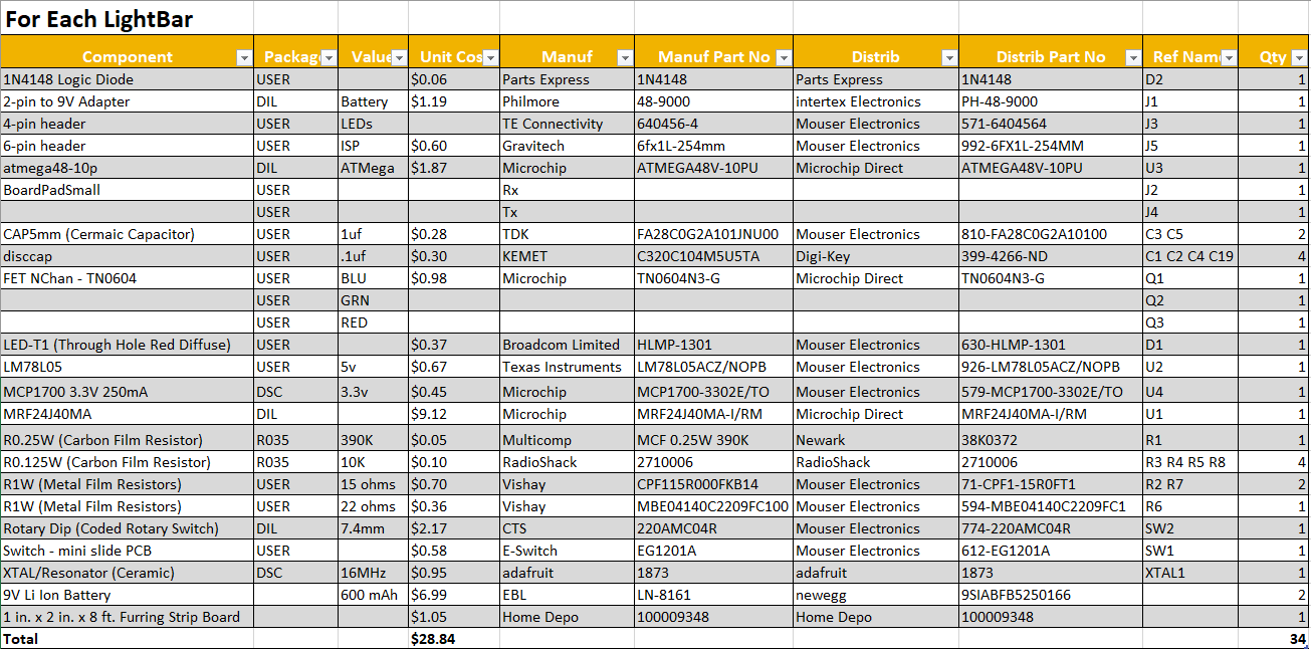
\includegraphics[width=160mm]{assets/Budget_Parts.png}
					\caption{Inventory Specifications and Contraints}
				\end{figure}
			
			\clearpage
			
		\section{Project Plan}
			
			\subsection{Team Roles and Responsibilities}
				\begin{itemize}
					\item \textbf{Budget Director:} Adrian Beehner
					\item \textbf{Client Liaison:} Kevin Dorscher
					\item \textbf{Designer:} Paul Martin
					\item \textbf{Documenter:} Andrew Butler\\
				\end{itemize}
			
				\noindent \textbf{Roles Were Selected/Assigned By:} Team consensus, with evaluating the strengths and weaknesses of teammates and accordingly assigning roles based on these. Discussion/volunteering for responsibilities will be the primary method, if this proves inefficient, a variation of team voting will be required.  Some roles will not be individual responsibilities however, but instead a collaborative effort that requires the professional coordination and responsibility of the entire team.
				
				\noindent \textbf{Responsibilities:} budget, primary contact client, organize team meetings, team documentation, scheduling, project management, onlien repository management, communication management, desigining, prototyping, testing, researching, diagrammming, analyzing, modeling, and manufacturing/assembly.
		
			\subsection{Schedule}
				The actual shchedule and the intended schedule differed greatly from one another. This is seen in the Gantt Chart figure shown in the Appendices. When examining the task of "Planning/Adjustments", it is clear that we did not reach our one month goal, as it led into October. While it was assummed this task would be simple, it provided a challenge to understand and coordiate the scope of the project. Hardware decisions became problematic, as it was only halfway finished by the end of October as seen in the Gannt chart, this wasn't entirely resolved until the beginning of december. The most problematic task that did not acoomplish its inteneded schedule is "Hardware Implementation", as for the month of Novemeber, only about 35 percent of it was accomplished. Partially due to the fact that other tasks were brought into the following months. The "Prototype and Unit Testing" task had the same issue. Evalutation didn't take much time, as the core design of the product was favorable, only lasting into the next month to finalize items. The "Produce Final Hardware" task went smoothly after the issues of prototyping and hardware implementation was accomplihsed, with the intented time being met. The "Hardware Scale and Software" task unexpectdly took more time, purely due the software being more elaborate and complex than orignally anticipated. "Testing" task for the product was fiarly simple, so intended and actual time had no differences. Finally the "Ship/Maufacture" task went smoothly, purely since the the client had fairly small needs/requirements for the process. 		
				
				\newpage
		
		\section{Concepts Considered}
		
				\subsection{Battery Design}
				The list below discusses the attributes for the battery specification, including the requirements, battery chemistry, voltage/capacity, and options/alternatives. Figures "9V Battery Design Specification" and "18650 Lithium Ion Battery Design Specification" corresponding to this information are found in Appendix B.
				
				% Remove Bullets from item list
				{\renewcommand\labelitemi{}
					% Begin list
					\begin{itemize}
						\item \textbf{Requirements}
						\begin{itemize}
							\item Battery required to power the LightBar for TowerOfLights
							\item 3 LEDS on LightBar requires 800 mA
							\item Voltage must be within the range of 8.6 – 9.3 V (Charge)
							\item 10.5 V to run 3 LEDs in a series
							\item 7V for 2 LEDs in a series
							\item Microprocessor based wireless Module distributes the power supply to LEDs on each board
						\end{itemize}
						\item \textbf{Chemistry}
						\begin{itemize}
							\item \textbf{Lithium Ion:} rechargeable battery type, due to high energy density, tiny memory effect, and low self-discharged, lithium ions move from negative electrode during discharge, and back when charging
							\item \textbf{Alkaline:} Popular primary battery (non-rechargeable), dependent on reaction between zinc and manganese dioxide
						\end{itemize}
						\item \textbf{Voltage/Capacity}
						\begin{itemize}
							\item Each LED requires around 3.5 V and each color takes 270 mA
							\item A 9 V battery could support two LEDs in a series, 9V batteries support a wide range of mAh, generally from 400-700 mAh
							\item A 18650 Battery, which has 3.7 V, can be placed in a 18650 holder for 3 batteries, providing 11.1 V, enough to power 3 LEDs in a series (current LightBar setup), with 18650 supporting a range of 1600-3600 mAh
						\end{itemize}
						\item \textbf{Options/Alternatives}
						\begin{itemize}
							\item \textbf{18650 Battery:} large capacity (mAh), allowing LEDs to run longer and can be configured to run LEDs in a series, if making battery pack from these, but requires long charging
							\item \textbf{9V Battery:} Provides smaller capacity, but faster recharge rate. Can only run 2 LEDs for a single 9 V
						\end{itemize}
						\item \textbf{Diagrams}
					\end{itemize}

		
			\subsection{Arduino / Receiver Design}
				
				\textbf{Arduino / Receiver Design Specifications} - Refer to figure in Appendix B - "Arduino / Receiver Design Specification"
				\begin{itemize}
					\item Multiple Arduino Atmega 328P boards fitted with a shield and attached receiver chip 
					\item Programming of the individual Arduino Atmega 328P boards using the Arduino IDE (C++)
					\item Receiver chip will delegate the sleep or wake-up modes for each individual light bar
					\item Receiver will also handle input from the transmitting X-Bee, and output data to the LED driver circuit
					\item Creation of the LED Driver circuit which will modify voltage as requested by each set of LED’s to provide a constant current power flow
					\item After modifying voltage accordingly, the LED driver circuit will output the data stream from the receiver to the network that each Arduino Atmega 328P is connected to
				\end{itemize}
			
			\subsection{LED Design}
				LED specifications and 2 potential solutions detailed below, these describe the requirements and proposed solutions/ideas.
				
				% Remove Bullets from item list
				{\renewcommand\labelitemi{}
					% Begin list
					\begin{itemize}
						\item \textbf{Specifications}
						\begin{itemize}
							\item 3 LEDs of each color (red, green, blue) per room
							\item Uses constant current (270-300 mA)
							\item Red LEDs drop ~2.5V per diode
							\item Blue and green LEDs drop ~3.5V per diode
							\item Colors are displayed with pulse-frequency modulation, as each diode can only be fully on or fully off at any moment
						\end{itemize}
						\item \textbf{Circuit Options}
						\begin{itemize}
							\item \textbf{Series} - Refer to figure in Appendix B - "Circuit diagram with LEDs in series"
							\item \textbf{Parallel} - Refe to figure in Appendix B - "Circuit diagram with LEDs in parallel"
						\end{itemize}
					\end{itemize}
					% Create new Page (NEED TO USE clearpage because we have pictures that will affect it!)
				
			%Wireless Design Spec
			\subsection{Wireless Design}
				
					% Remove Bullets from item list
					{\renewcommand\labelitemi{}
						% Begin list
						\begin{itemize}
							\item \textbf{Frequency Requirements}
							\begin{itemize}
								\item The wireless protocol needs to have an effective range of potentially up to 100 meters. Additionally, the
								frequency must be one that will work even in crowded venues, with lots of different cellphones, and
								Wi-Fi signals present.
							\end{itemize}
							\item \textbf{Speed Requirements}
							\begin{itemize}
								\item The wireless protocol needs to have the ability to send enough data fast enough to keep up with the
								Tower Lights show. Depending on the total number of light-bars, this number can change. The speed
								requirement will also depend on how many possible colors we implement and how many frames per
								second we will display.
							\end{itemize}
							\item \textbf{Packet Requirements}
							\begin{itemize}
								\item The information packets sent over the wireless protocol must contain all the information needed to set
								the individual light bars to the appropriate color. There can be only one packet that will be sent to all
								the light bars, and each light bar will be encoded with which part of the packet to read.
							\end{itemize}
							\item \textbf{Potential Solution} - Refer to Appendices for figure coressponding to "Zigbee Wireless Protocol" caption
							%\begin{itemize}
							%\item Zigbee Protocol
							%\end{itemize}
						\end{itemize}
		
			\subsection{LightBar Design}
			
			\textbf{Wooden Structure}
			The figure in the Appendices with the caption "Model of LightBar" coresponds tot he design of the Lightbar. The Lightbar is essentially a 1inX2in board the houses a battery, and the LEDs in either series/parallel, the LED Driver Circuit. This concept originates from the orignal TowerOfLights porject, which also utilized this design, mainly for its cost effectivness and easy mobility and structual integrity. Cheap, easy to obtain are the main draws of the item. The look of the LightBar itself however is not professional, to a large extent, although client never seeked a revisioned look on the LightBar.
			
				%\begin{figure}[!htb]
					%\centering
					%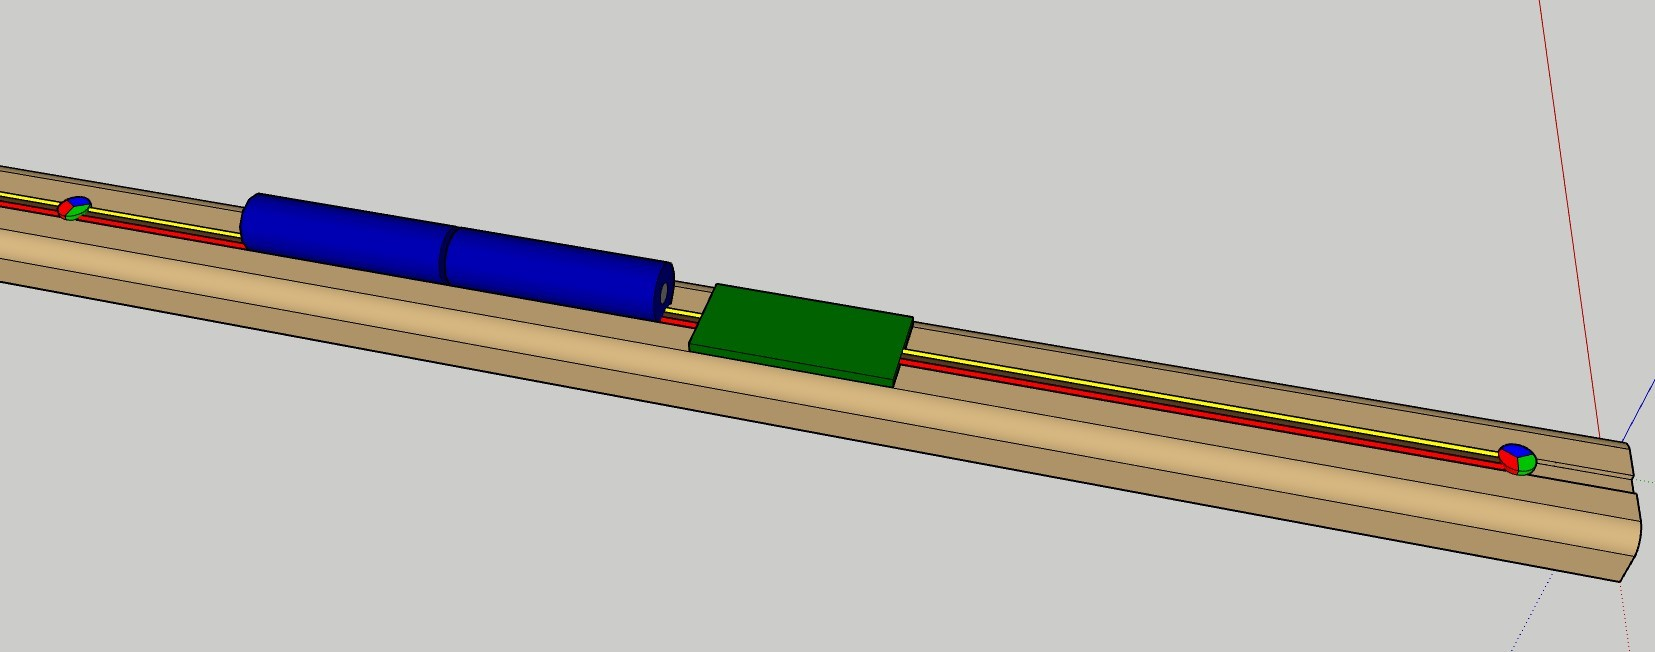
\includegraphics[height = 50mm]{assets/Lightbar_Model.jpg}
					%\caption{Model of LightBar \label{overflow}}
				%\end{figure}
			
			\noindent \textbf{3D Printered Structure}
			Conceptually, that same figure mentiond above, althouh representing the wooden LightBar model, there was decision process as whether or not a 3D printed structure would be plausible, or at least to some extent holders for various components. This would allow cost effective designs, however its greatest hiderence is time and location, as the only readily avilable 3D Printer neeed for such as task was located at Unievrsity of Idaho's CDA CS location. The time of each lightbar print would also take upwards of 24 hours, based on this figure above. The 3D printer would provide a more professional look to the item.
			
			\newpage
	
	\section{Concept Selection}
	The method to decide which concepts to use in the product were done through the use of decision matrices. These matrices helped outlined the specific pros and cons of each design, while providing a thoughful score. The following sections outline the selections chosen, via reference to the decision matrices.
	
		\subsection{9V Battery vs 18650 Battery}
			
			\noindent\textbf{Conclusion}\\
				The final decision was to utlilze a 9V Battery. The decision matrix of this reasoning is shown in the figure below.
				
				\begin{figure}[ht!]
					\centering
					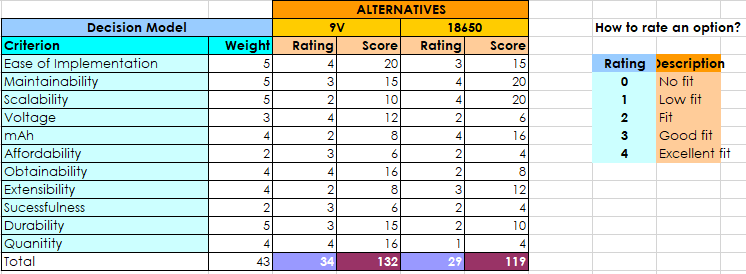
\includegraphics[width=120mm]{assets/9V_vs_18650.png}
					\caption{9V vs 18650 Battery \label{overflow}}
				\end{figure}
		
		\subsection{Series vs Parallel Circuit}
			The final decision was to utilize a parallel circuit. The decision matrix of this reasoning is shown in the figure below.
			
			\begin{figure}[ht!]
				\centering
				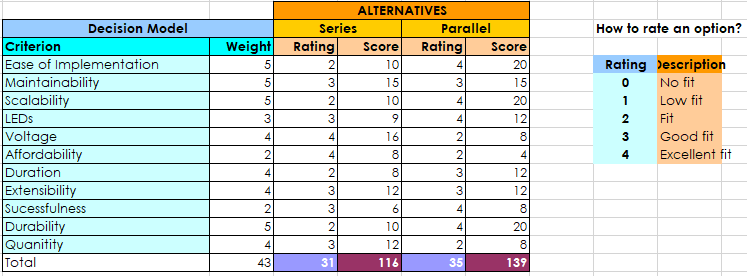
\includegraphics[width=120mm]{assets/Series_vs_Parallel.png}
				\caption{Series vs Parallel Circuit \label{overflow}}
			\end{figure}
		
		\subsection{WoodenLightBar vs 3D Print}
			The final decision was to utilize the wooden 1inx2in board for the LightBar. The decision matrix of this reasoning is shown in the figure below.
			
			\begin{figure}[ht!]
				\centering
				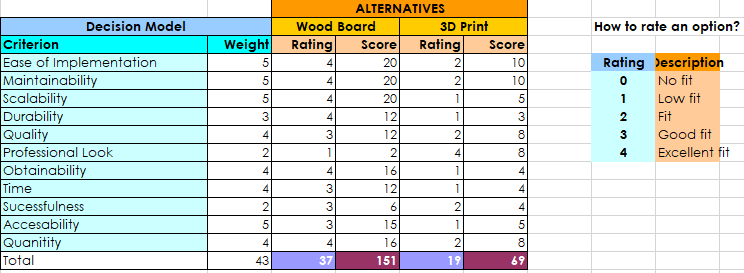
\includegraphics[width=120mm]{assets/Wood_vs_3D}
				\caption{Wooden LightBar vs 3D Printed LightBar \label{overflow}}
			\end{figure}
			
		\subsection{Other Final Selections Process}
		The other choices, such as the 805.15.4 protocol, were galringly obvious choices or requested concepts from the sponder. These additional concepts neiher presented nor warrented further dicsussions/ diagrams/ decision matrices, or morphological charts on the matter. 
		
		\newpage
		
		
	\section{System Architecture}
	
		\subsection{Proof of Design}
		A discussion of the various components is shown below, providing evidence of components working together.
		
		% Remove Bullets from item list
		{\renewcommand\labelitemi{}
			% Begin list
			\begin{itemize}
				\item \textbf{LightBar}
				\begin{itemize}
					\item LightBar designed similar to original "Tower of Lights" one
					\item 1 in x 2 in
					\item Size supports common sizes that are used for PCBs and LEDs
				\end{itemize}
				\item \textbf{LED Driver Circuit}
				\begin{itemize}
					\item Similar to "Goofy Glasses" Circuit
					\item Schematic will be very similar, besides the fact that higher voltage and some other additional items will be added
				\end{itemize}
				\item \textbf{Towerplayer Program}
				\begin{itemize}
					\item Modified from various files from original "Tower Player" programs:
					\begin{itemize}
						\item towerarduino.ino
						\item towerplayer.cpp
						\item yswavfile.cpp
						\item yswavfile.h
					\end{itemize}
				\end{itemize}
				\item \textbf{LED}
				\begin{itemize}
					\item LEDs already function on "Goofy Glasses"
					\item Similar design, with battery and circuit providing the power and data to correctly display specific color for LED
					\item Layout of LEDs will actually follow similar design as the original "Tower of Lights" LightBar.
				\end{itemize}
				\item \textbf{Battery}
				\begin{itemize}
					\item 9V Lithium Ion Battery already working on Goofy Glasses
					\item Currently provides 30 minutes of run time
					\item Current Battery choices are between 9V Lithium Ion and 18650 (which would last longer)
				\end{itemize}
			\end{itemize}
			
			A diagram that correlates to the information that is provided above discussing the proof of design id shown below. Images are provided in the diagram to help provide a visual for certain aspects.
			
			\begin{figure}[!htb]
				\centering
				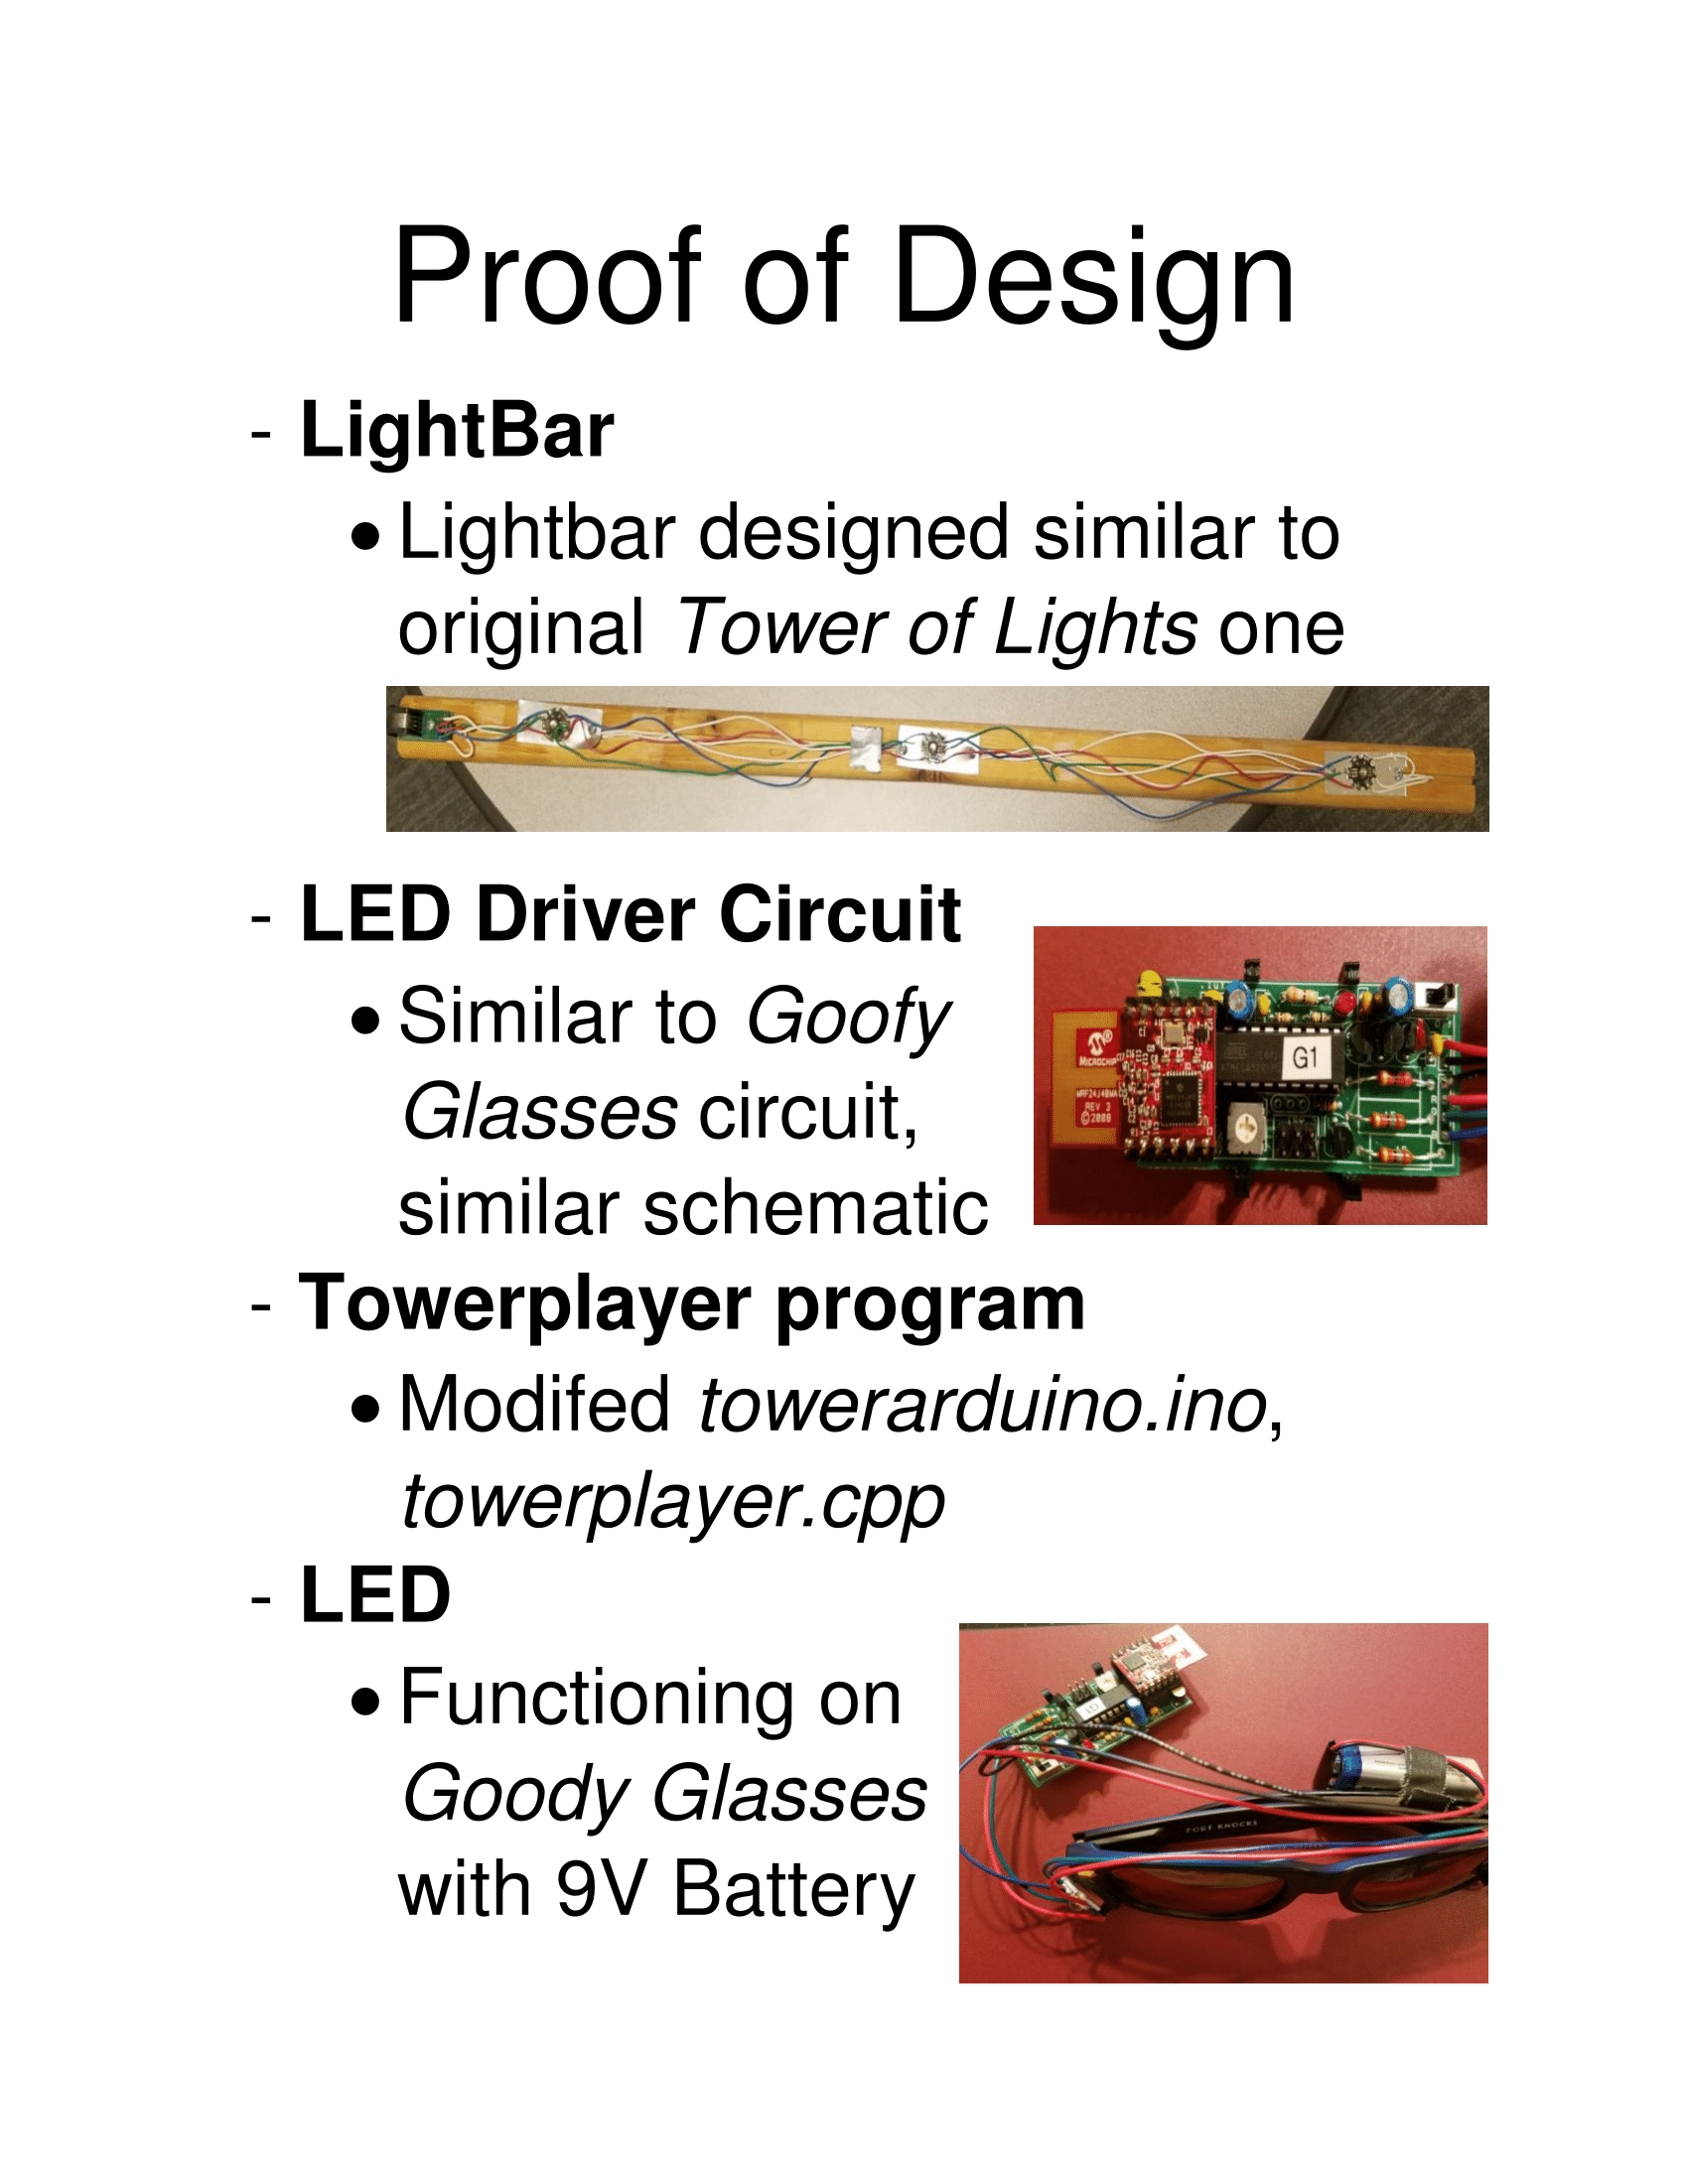
\includegraphics[width = 70mm, height = 80mm]{assets/Proof_Of_Design.png}
				\caption{Proof of Design \label{overflow}}
			\end{figure}
			
				
		\subsection{Current Product}
			The current product flow in regards to the final product is shown below in Figure below. The current setup does not have any battery setup, and requires a wired connection. Changing this is the core of this project, which will improve the versatility of the TowerOfLights product.
			
			\begin{figure}[ht!]
				\centering
				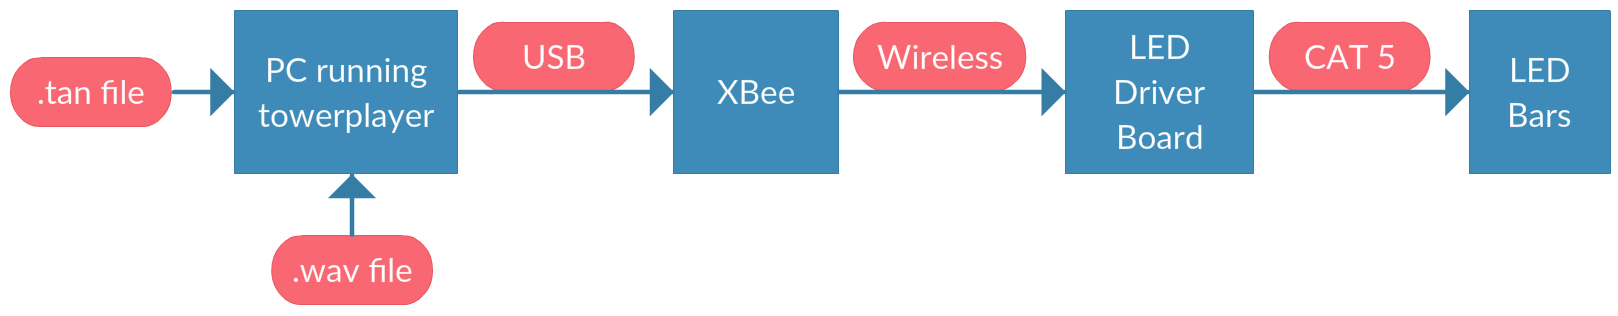
\includegraphics[width=170mm]{assets/What_We_Have.png}
				\caption{Current Product Flow \label{overflow}}
			\end{figure}
		
		
		\subsection{Desired Product}
			The desired product flow is shown in the figure below. The main focus is on the battery that should power each Arduino reciever, as well as the SPI protocol from XBee to the Receiver. This is to make the process wireless instead of wired, which is the main goal of this endeavor, helping to justify the system architecture of the product.
			
			\begin{figure}[ht!]
				\centering
				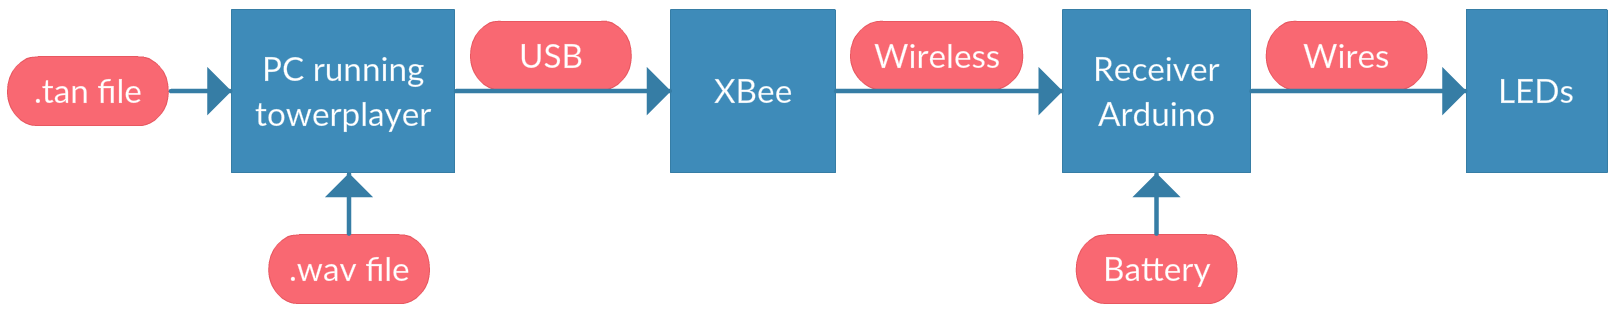
\includegraphics[width=170mm]{assets/What_We_Want.png}
				\caption{Desired Product Flow \label{overflow}}
			\end{figure}
		
		
		\subsection{PC Running TowerPlayer}
		The diagram for a flow chart depicting the sequence of actions for running the TowerPlayer program on a computer is shown in the figure below. This diagram helps with understanding the underlying software that needs to be setup and used before the hardware can successfully work together. It also demonstrates and justifies the system architecture of the project.
		
		\begin{figure}[ht!]
			\centering
			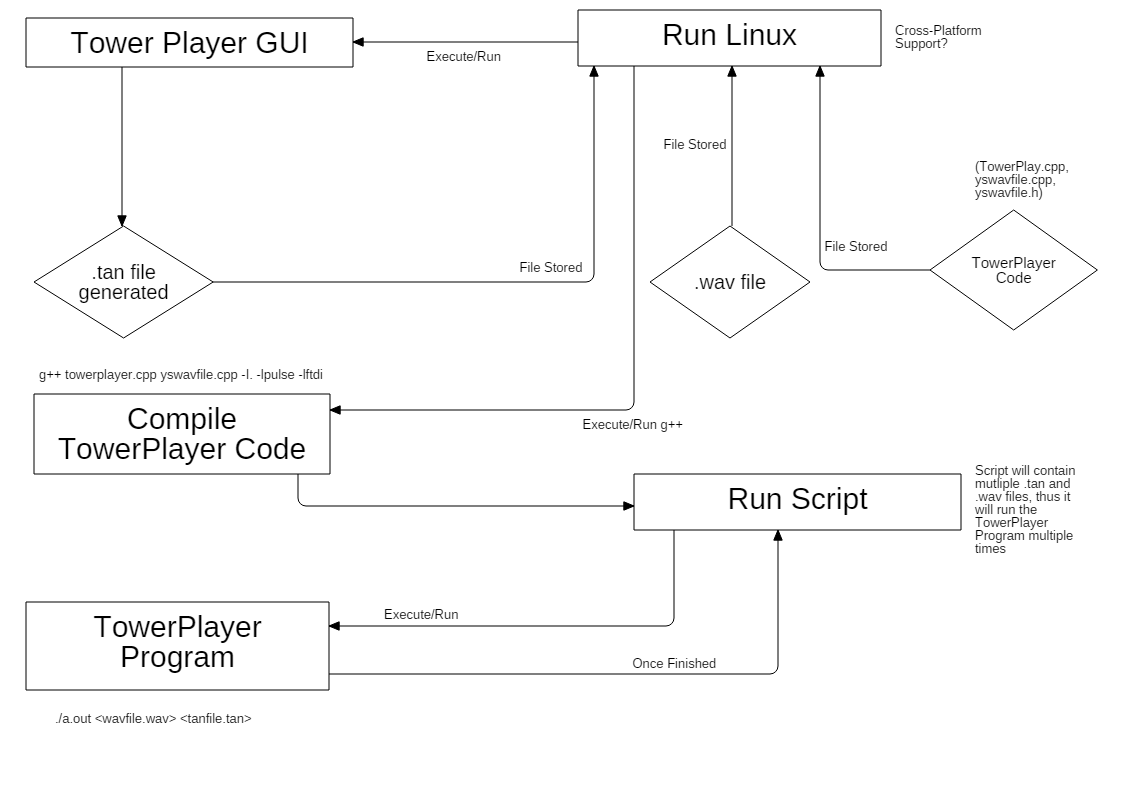
\includegraphics[width=150mm]{assets/PCRunningTowerPlayerFlowChartDiagram.png}
			\caption{Flow Chart Diagram for PC Running TowerPlayer \label{overflow}}
		\end{figure}
	
		\clearpage
		
		
	\section{Design Evaluation}
	Please refer to the Appendex "DFMEA Worksheet" for additional/corresponding information below.
	
		\subsection{DMFEA vs Project Specifications}
			\textbf{Wireless LightBar System:} The Wireless LightBar system's met the project specifications required by the client, with a risk priority of 1. The focus of the entire system was to make sure the user was able to utilize the system correctly. There were mainly only two way that the Light Bar could fail at this point, either the computer itself was not set up correctly, or the LightBar itself had failed to be assembled correctly. Every other issue with fail into the failures of the other major of components listed in the DMFEA. The dsign risks itself for the LightBar are mainly the components being fairly loose, but eve thought testing, the issue never arose. The best remedial action was thus to just make clear directions for user.\\ \\
			\textbf{LightBar:} The actual LightBar is the key of the product, and met the project's specifications, while being fairly low risk priority on the DFMEA. The reason was mainly due to very little requirement from the project specification, thus the LightBar could have precuations made to reduce risk. The only symptom of failure of the LightBar is that it fails to operate, thus no lights/effects come from the bar itself. There were two issues from this either computer error, or wireless protocol error, or user error. The team only ran into the user error one, by putting dead batteries into the lightbar. Thus the risk prioirty for this component was only 1. The remedial action was then to simply warn users of wireless protocol and computer errors.\\ \\
			\textbf{TowerPlayerProgram:} The TowerPlayerProgram is another key aspect to the product, the main specifications of the program were to meet the low-power mode settings and also split the 32 channels into 64. This was succeeded without making the failure/risk increase on the DFMEA. This is due the fact the only failure that can occur is that the program, which is loaded onto the LightBar cannot send data (thus the Lightbar shows nothing). The two reasons for this is computer user error (not running program correctly), or wireless protocol error, both which the team tested and never occured. Thus due to the low frequency of it happening, and its low severity, the risk prioity is 1, the lowest risk. The remedial action is to inform the user of requried libaries/software needed to use program.\\ \\
			\textbf{TowerArduinoProgram}: The TowerArduinoProgram is another key piece of software, function like the previous item. The same exact risks and issues that plague the TowerPlayer. There is on difference, mainly in that instead of the failure likely coming from comotuer user error, it comes from manufacturing error of incorreclt using Adruino IDE, and thus the program is not flashed onto the AtMega328P. However the issues both are similar, and software posses low risks, and thus risk priority is 1 again. The remedial action is to inform the user of requried libaries/software needed to use program.\\ \\
			\textbf{LED Driver Circuit:} The LED Driver circuit is one of the core aspects of the product, essentially communicating to LEDs to produce the lightshow. Thus this circuit has a much higher risk than the other components. The project specifications also constrained and hampered this issue further, as it was required that each LightBar have its own microcontroller, which means that every LightBar is at high risk for this component. The failure of the LED Driver Circuit can only amount from the crcuit becoming damaged/soldered incorrectly. Both of these failures have almost never occured in testing, however, these circuits, if damaged or not manufactured correctly can be harmful. The harmfulness of these circuits is why it gets a severity of risk at 4, the highest, as there is a very high likelyhood that if a circuit malfunction it could cause harm, or create a fire hazard. Thus the risk priority of the LED Driver circuit is a 4. The only remiedal action is a hazard and danger warning on product. \\ \\
			\textbf{Other Components:} All other components are purchased and manufactured elsewhere and are extremely simple, thus the only possible failure that can occur is component failure. These components almost all follow the project speficificaitons laid out, such as power on/off state, a microporcoessor, receiver chip, and so on. These requirements factored into a higher risk for the lightBar, as having more need created higher risks in many areas. Some component failures provide less risk than others. The main risk contenders are the logic dinodes, 4-pin headers, capacitors, transistors, resistors, and 9V lithium Ion battery. Since these products are past team's control, can at most add "warning" label to product, mentioning each piece's risk.
		
		
		\subsection{Testing Procedures}
		The testing procedures utilized in the project were fairly simple but provided stable data to understand the sucess of the components.
		
			\noindent \textbf{LED Driver Circuit:} To test the circuit, a mutilmeter was to used to make sure the grounds are all 1 continuous circuit, and then test the power output to make sure the voltage level is correct with the schematic.\\
			Another test was turning on the power switch and looking for the red Diode to turn on, signfiying correct power.\\
			To test everything on circuit, the circuit was attatched to LightBar, LEDs, and flashed the towerarduino.ino program, and then send a demo code from ccomputer with receiver.
			
			\noindent \textbf{9V Battery:} Battery was tested by simply running the LightBar wiht a dmeo continuously, and timing the operation time and recharge time. Over 20 tests had been conducted on a 9V 600 mAh Lithium Ion Battery that had been rechared.
			
			\noindent \textbf{TowerArduinoProgram:} Program was tested by running out debugging information within the code itself, to see that correct information was being directly sent to receivers.
			
			\noindent \textbf{Transceivers and Receivers:} Only plausbile test was to run LightBar with dummy demo program.
	
		\subsection{Testing Results}
		Testing results were postive, and little to no surprises occured, the results were shown on multiple lightbars, each manufactured by different individual, and each on either different (same model, but not exact same battery) or recharged batteries.
		
				\noindent \textbf{LED Driver Circuit:} Circuit always functioned correctly, with no issues, besides user error. Test thorughly (around 20 times).
				
				\noindent \textbf{9V Battery:} Battery's operational time was 2 hours, exceeding client's need of 45 minutes. Testing done thoroughly (20 times).
				
				\noindent \textbf{TowerArduinoProgram:} Program achieved desired results were executed, tested thorughly (20 time), no issues.
				
				\noindent \textbf{Transceivers and Receivers:} Both always operated correctly with no issues, tested throughly (20 times). 
				
				\newpage
	
	\section{Future Work}
	
		\subsection{Recommendations for Adoption/Implemtation}
		The sponsor only requested around 4 prototypes of the LightBar, for effective and practical use, a multiude of LightBars will be requried. Additionally, the previous capstone project working on the graphical interface that produces tan files should be bundled with this product if applicable, as it would provide the user with the full versaility of a light show. The sponsor should examine the idea of sotring program data for light show into the microporocessor itself, still via the receiver chip. This may produce less latency, however it is noted at the same time team did not occur any major latency issues that would present an issue to current design. For actual setup of the system, 2-3 days in advance would be recommened, the day of the show shouldn't need to worry, since the LightBars will stay in low power mode. It may be worth the sponsor's time to enhance the convience of this system by looking into solar power, or another enegery option, however the difficulty and time involved may be sluggish and problematic. It is recommended that the sponsor follows up with any additional questions for team, if said question did not have an answer in the documenation, via the contact info listed on the cover page.
		
		\subsection{Missing Features}
		Missing features that did not make their way into the current design are prevelant, yet understand in the scope of the product. The only core feature that did not make it in that was desiried was cross-platform support (requested by client). At the moment, the program still only operates with Linux Operating Systems, and Mac OSX and Windows OS are not supported. Team ran into library issues and time contraints and made the decision of what feature could be omitted without sacrificing the core premise of the product. Other features missing would not be classified as missing, so much as "desired", as all other core features made their way into the design. 
		
		\subsubsection{Estimated Scope of Next Steps}
		The scope of the next steps is manufacuturing and assembly large scale, which depends on a variety of factors. The circuits themselves are not too complicated to produce and volunteers could easily help design a large magniutde and them and LightBars. The duration of this next steps primarily focueses on the labor willing to produce the LightBars, and the knowledge base. Essentially manufacturing and distrbuting this system to willing parties is the next step, with enought time, manpower, or both getting the system to willing consumers should be reasonable. Cost is difficult to estimate, for example,  Theophilus Tower Dormitory having 40 windows on one side, 40 LightBars time 30 dollars for each would estimate 1,200 dollars just for parts. Likely costs would range 1,000~3,000 dollars for a building. Labor costs (volunteer, professional, amateur) for producing LightBars is unknown however.
		
		\newpage
	
\appendix	
	\section{Calculations and Drawings}
	
		\subsection{Drawing of Original Schedule}
		Drawings produce during Team Meeting of orignal schedule
			\begin{figure}[!htb]
				\centering
				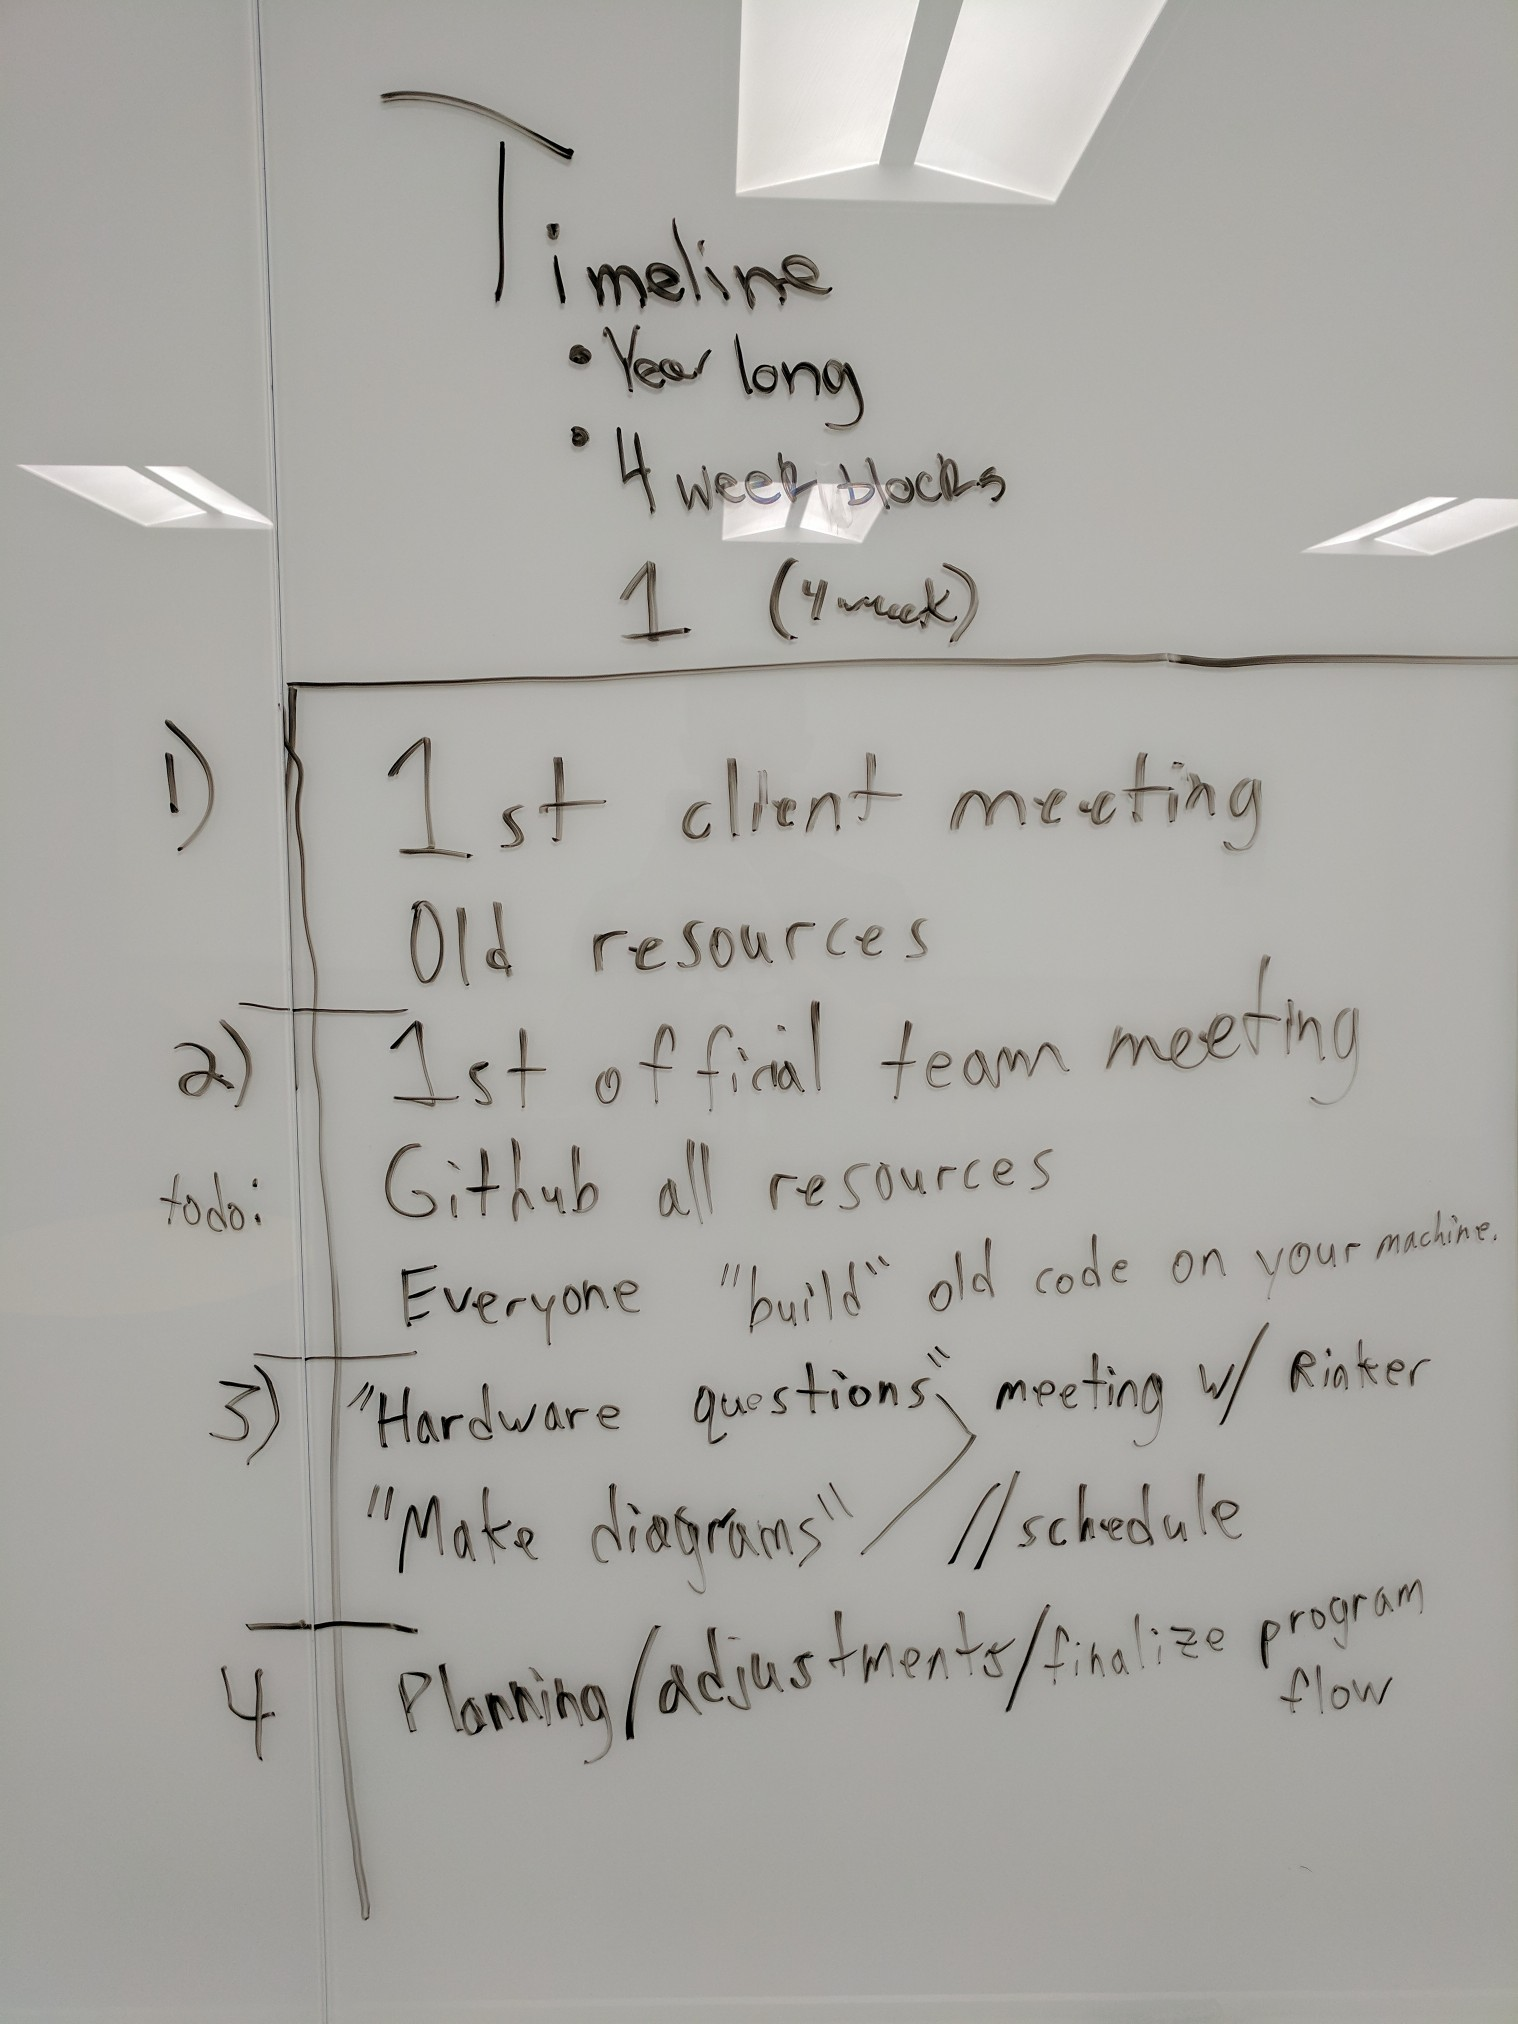
\includegraphics[width=100mm]{assets/9-14_Project_Agenda_1.jpg}
				\caption{9/14 Meeting Project Schedule \label{overflow}}
			\end{figure}
			
			\begin{figure}[!htb]
				\centering
				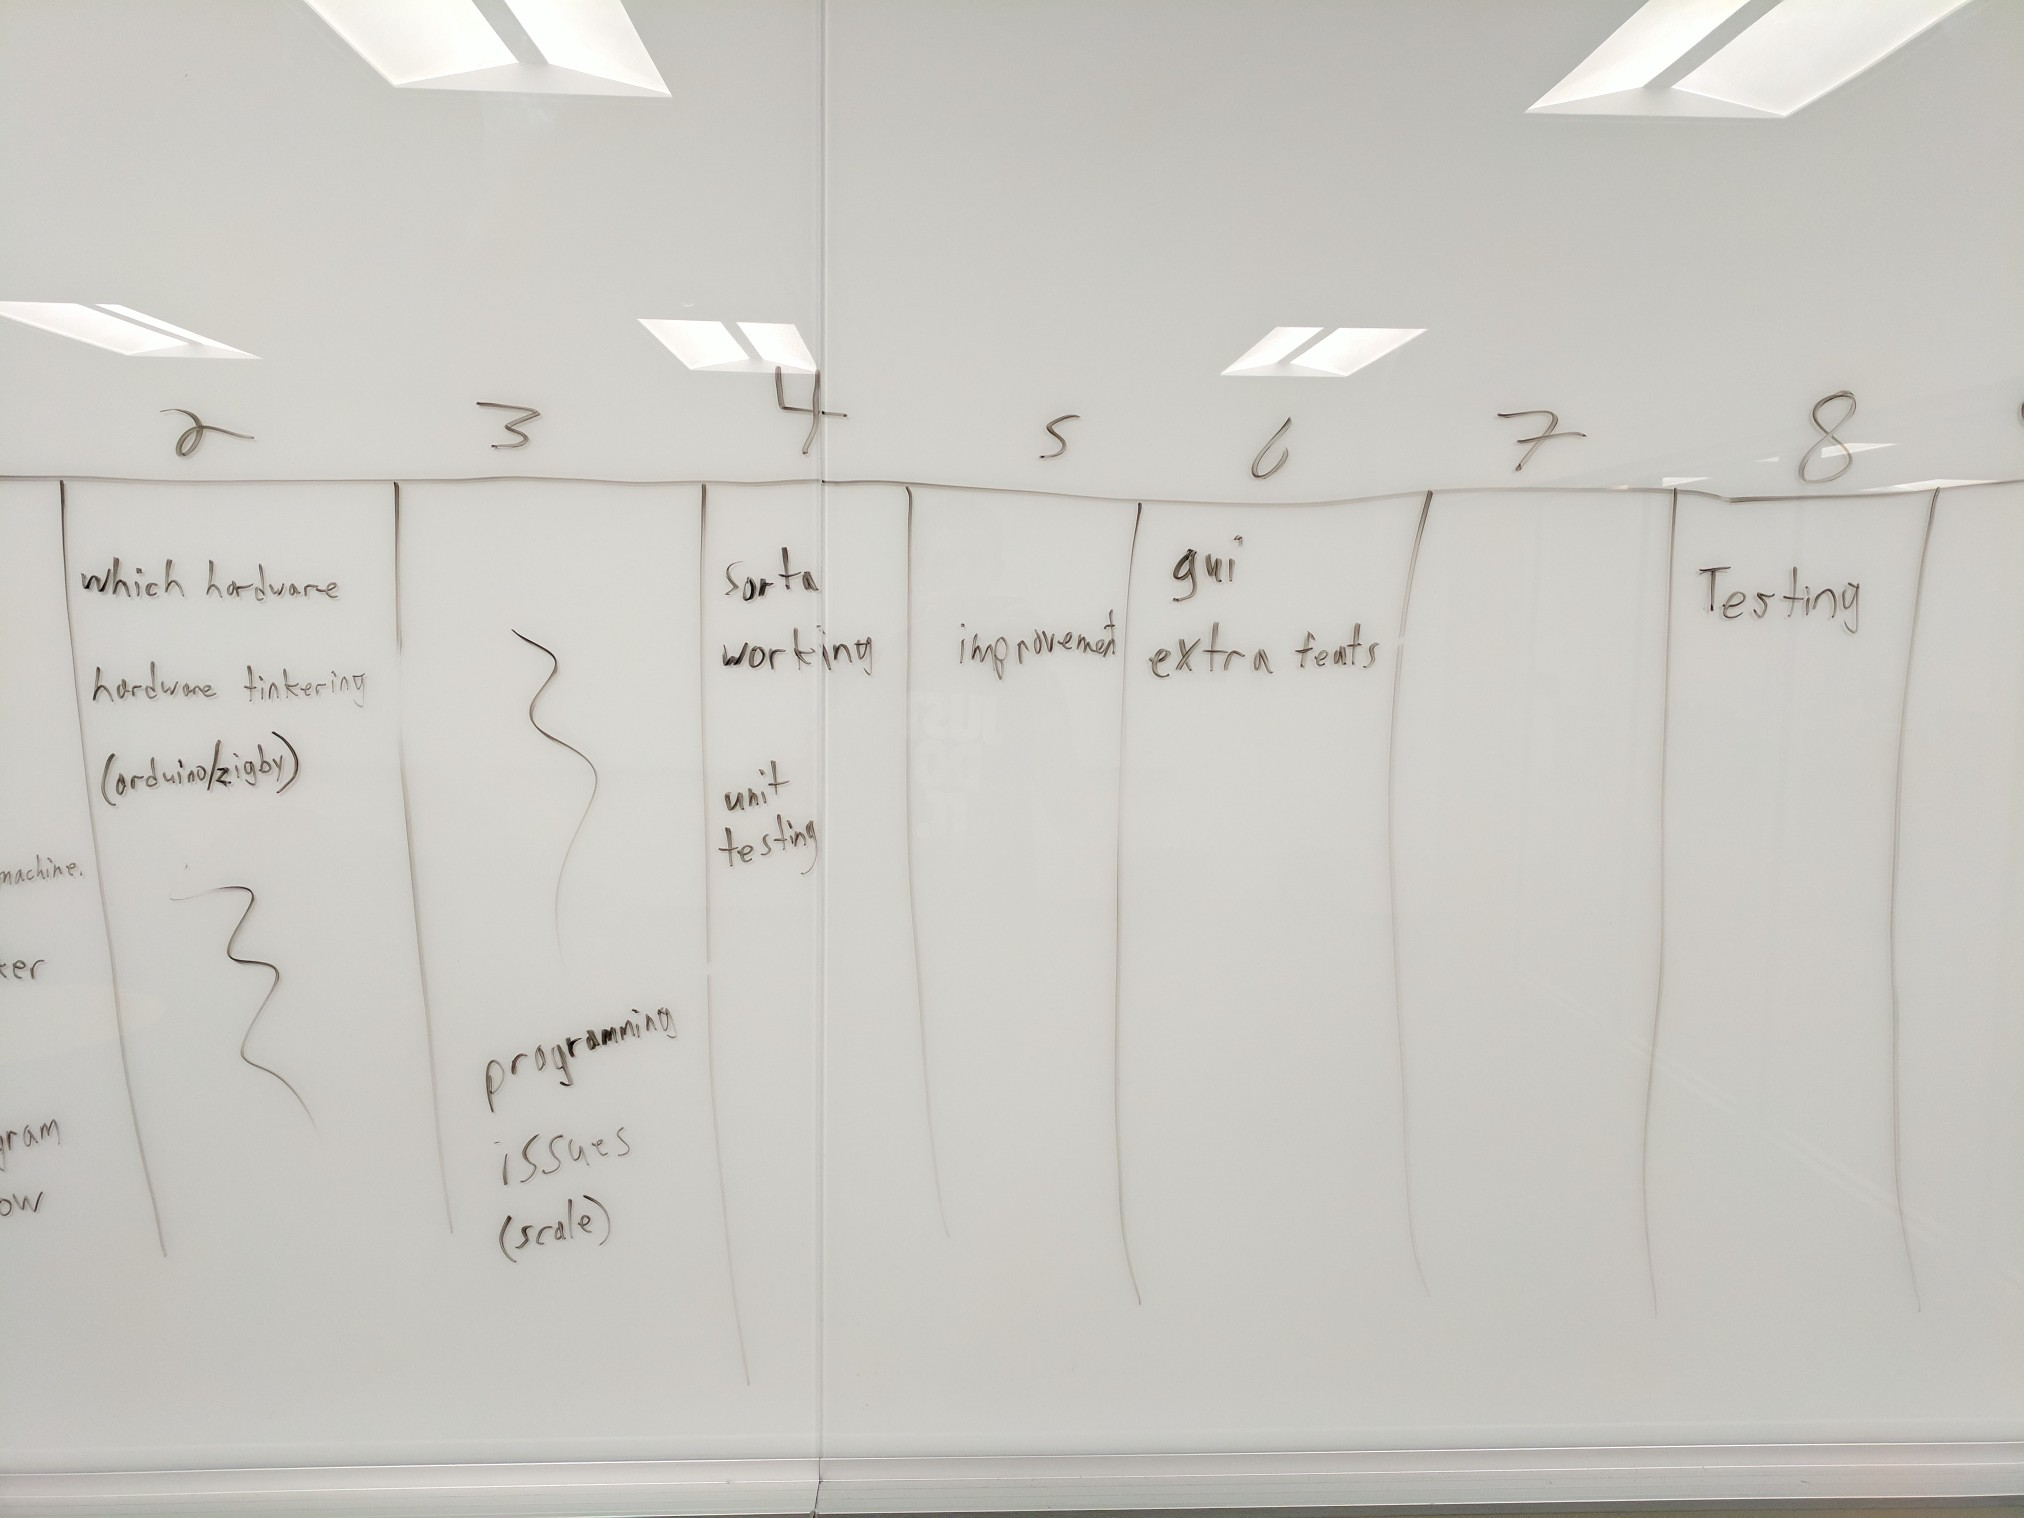
\includegraphics[width=100mm]{assets/9-14_Project_Agenda_2.jpg}
				\caption{9/14 Meeting Project Schedule \label{overflow}}
			\end{figure}
	
		\subsection{LightBar 3D Model}
		3D CAD Model of LightBar
			\begin{figure}[ht!]
				\centering
				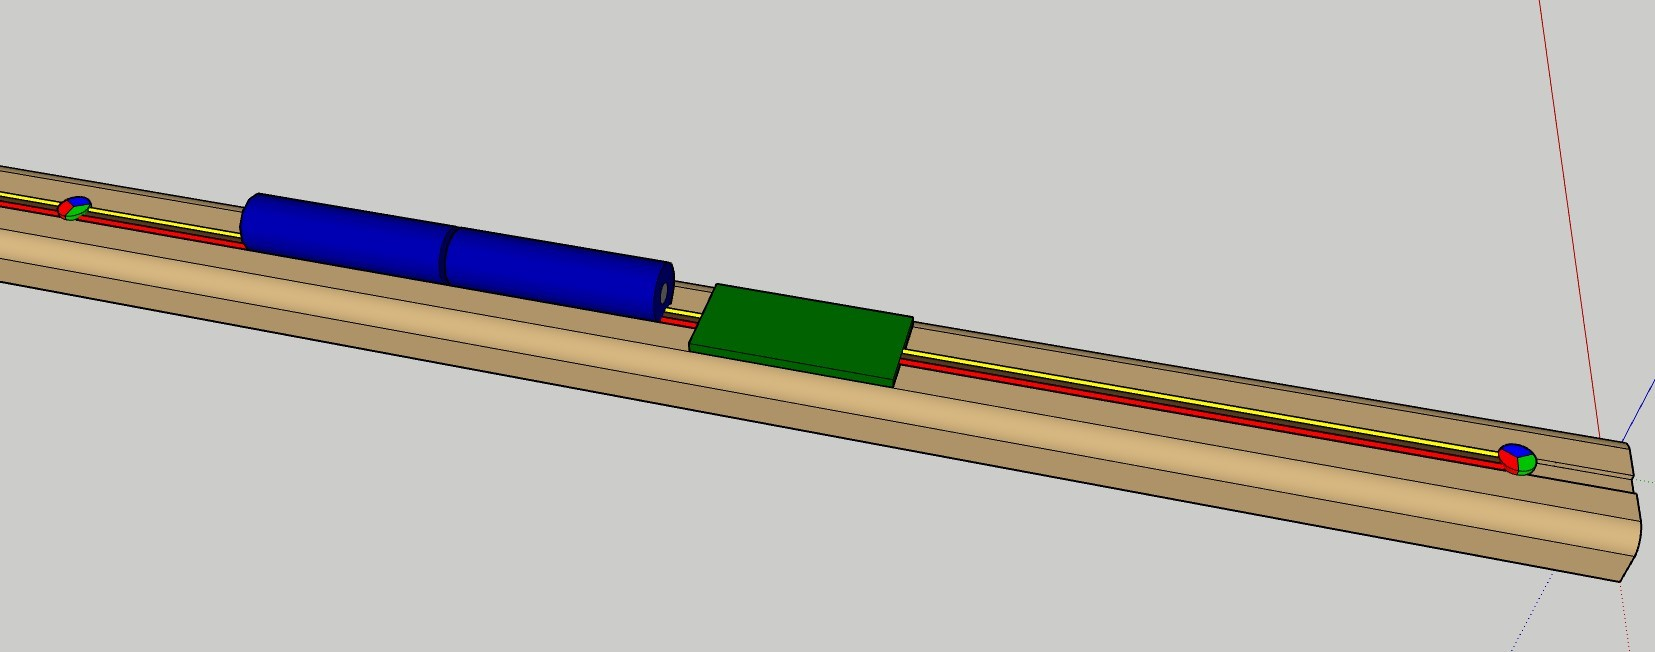
\includegraphics[width=170mm]{assets/Lightbar_Model.jpg}
				\caption{3D Model of Final Product \label{overflow}}
			\end{figure}

	\clearpage
	
	\section{Tables and Figures}
	
		\subsection{Arduino / Receiver Design Specification}
			The general diagram of the Arduino and reciever working together
			\begin{figure}[!htb]
				\centering
				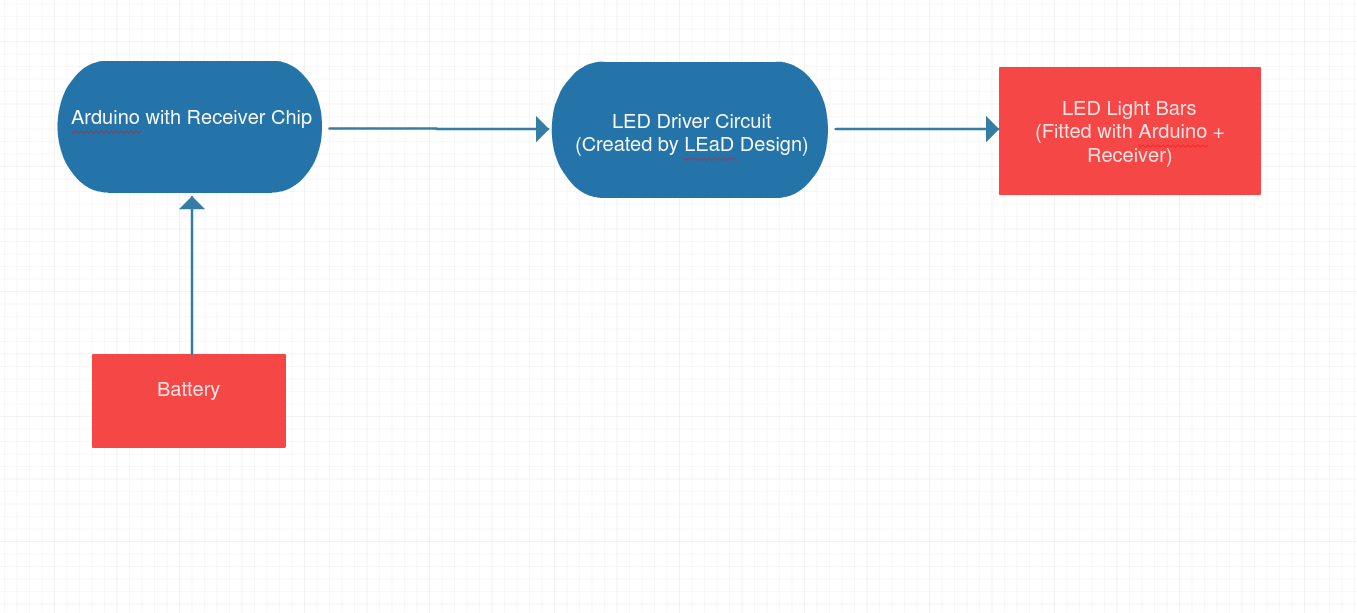
\includegraphics[width = 140mm, height = 60mm]{assets/Arduino_Receiver_Diagram.png}
				\caption{Arduino / Receiver Design Specification \label{overflow}}
			\end{figure}
		
		\subsection{Battery Design Specification}
			The diagrams containing the 9V Battery and 18650 Battery specifications.
			\begin{figure}[!htb]
				\centering
				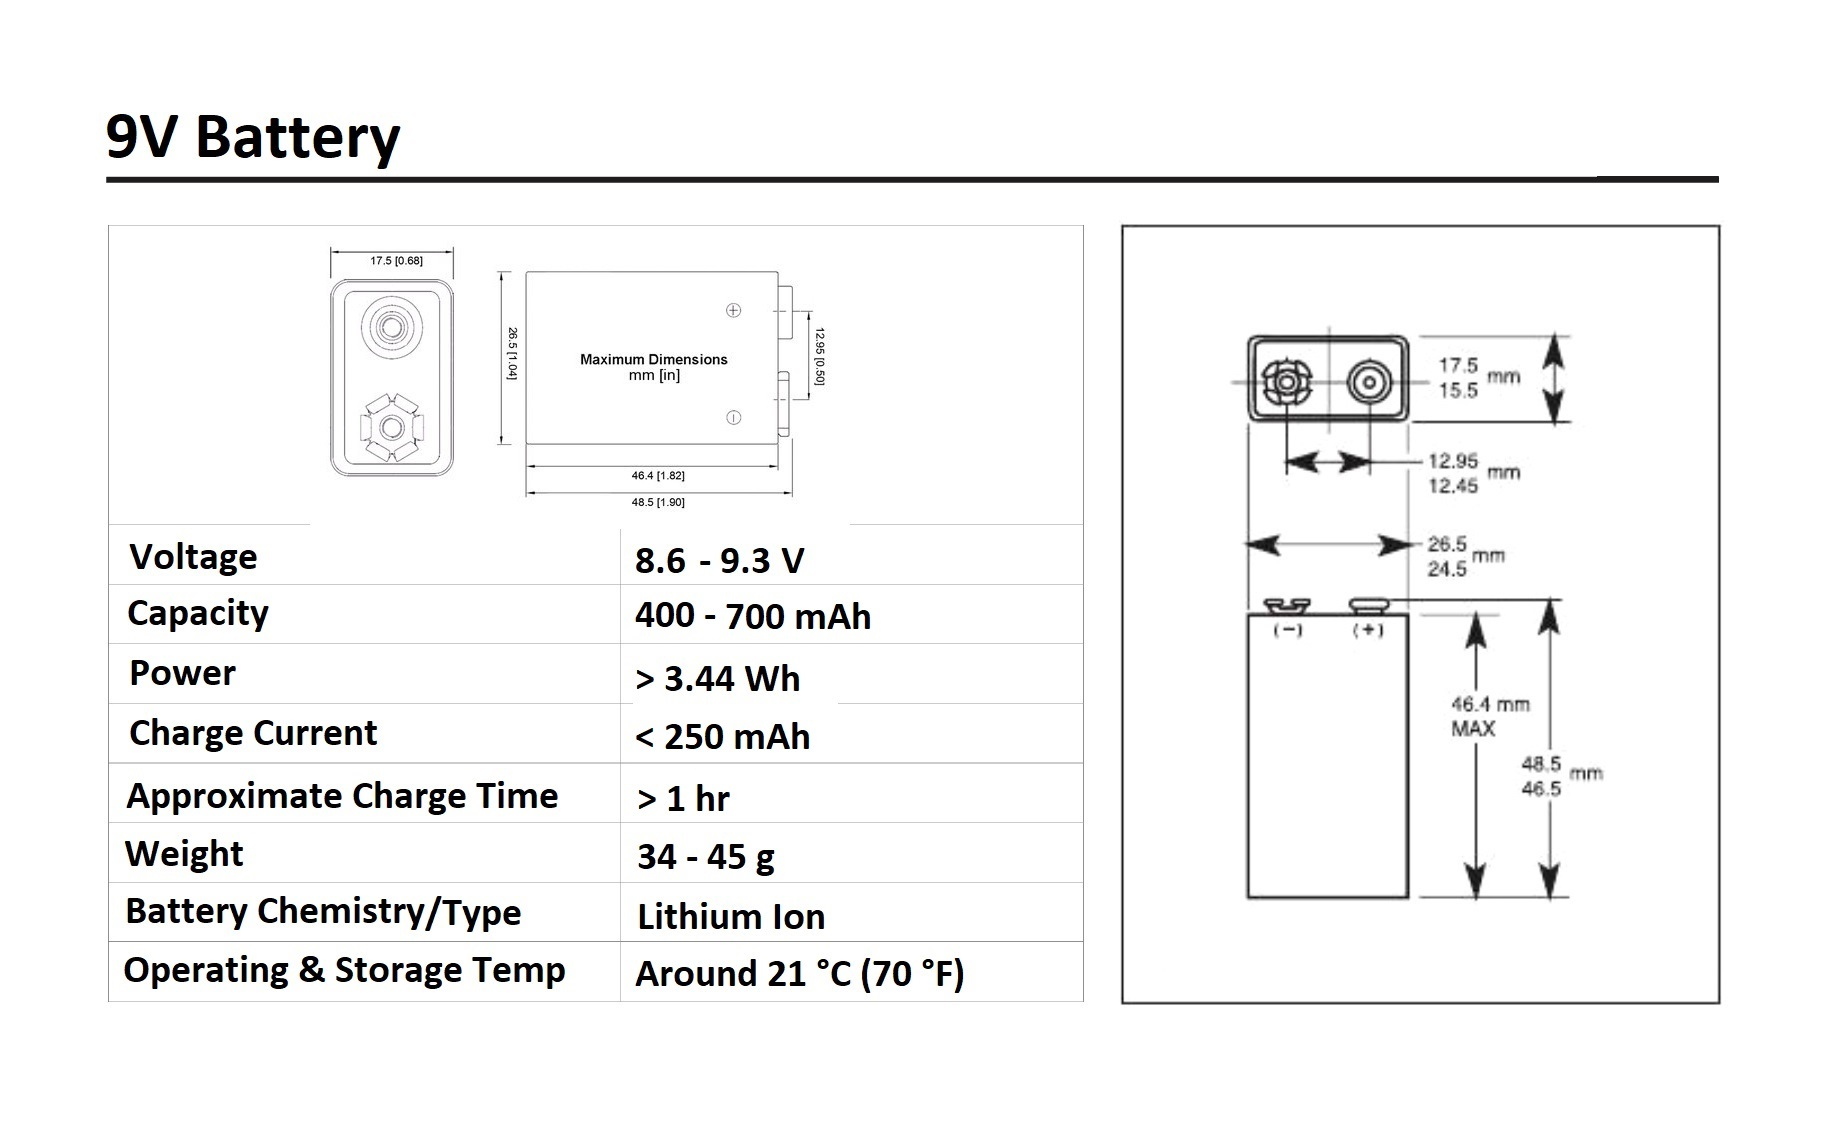
\includegraphics[width = 140mm, height = 80mm]{assets/9V_Battery.jpg}
				\caption{9V Battery Design Specification \label{overflow}}
			\end{figure}
			
			\begin{figure}[!htb]
				\centering
				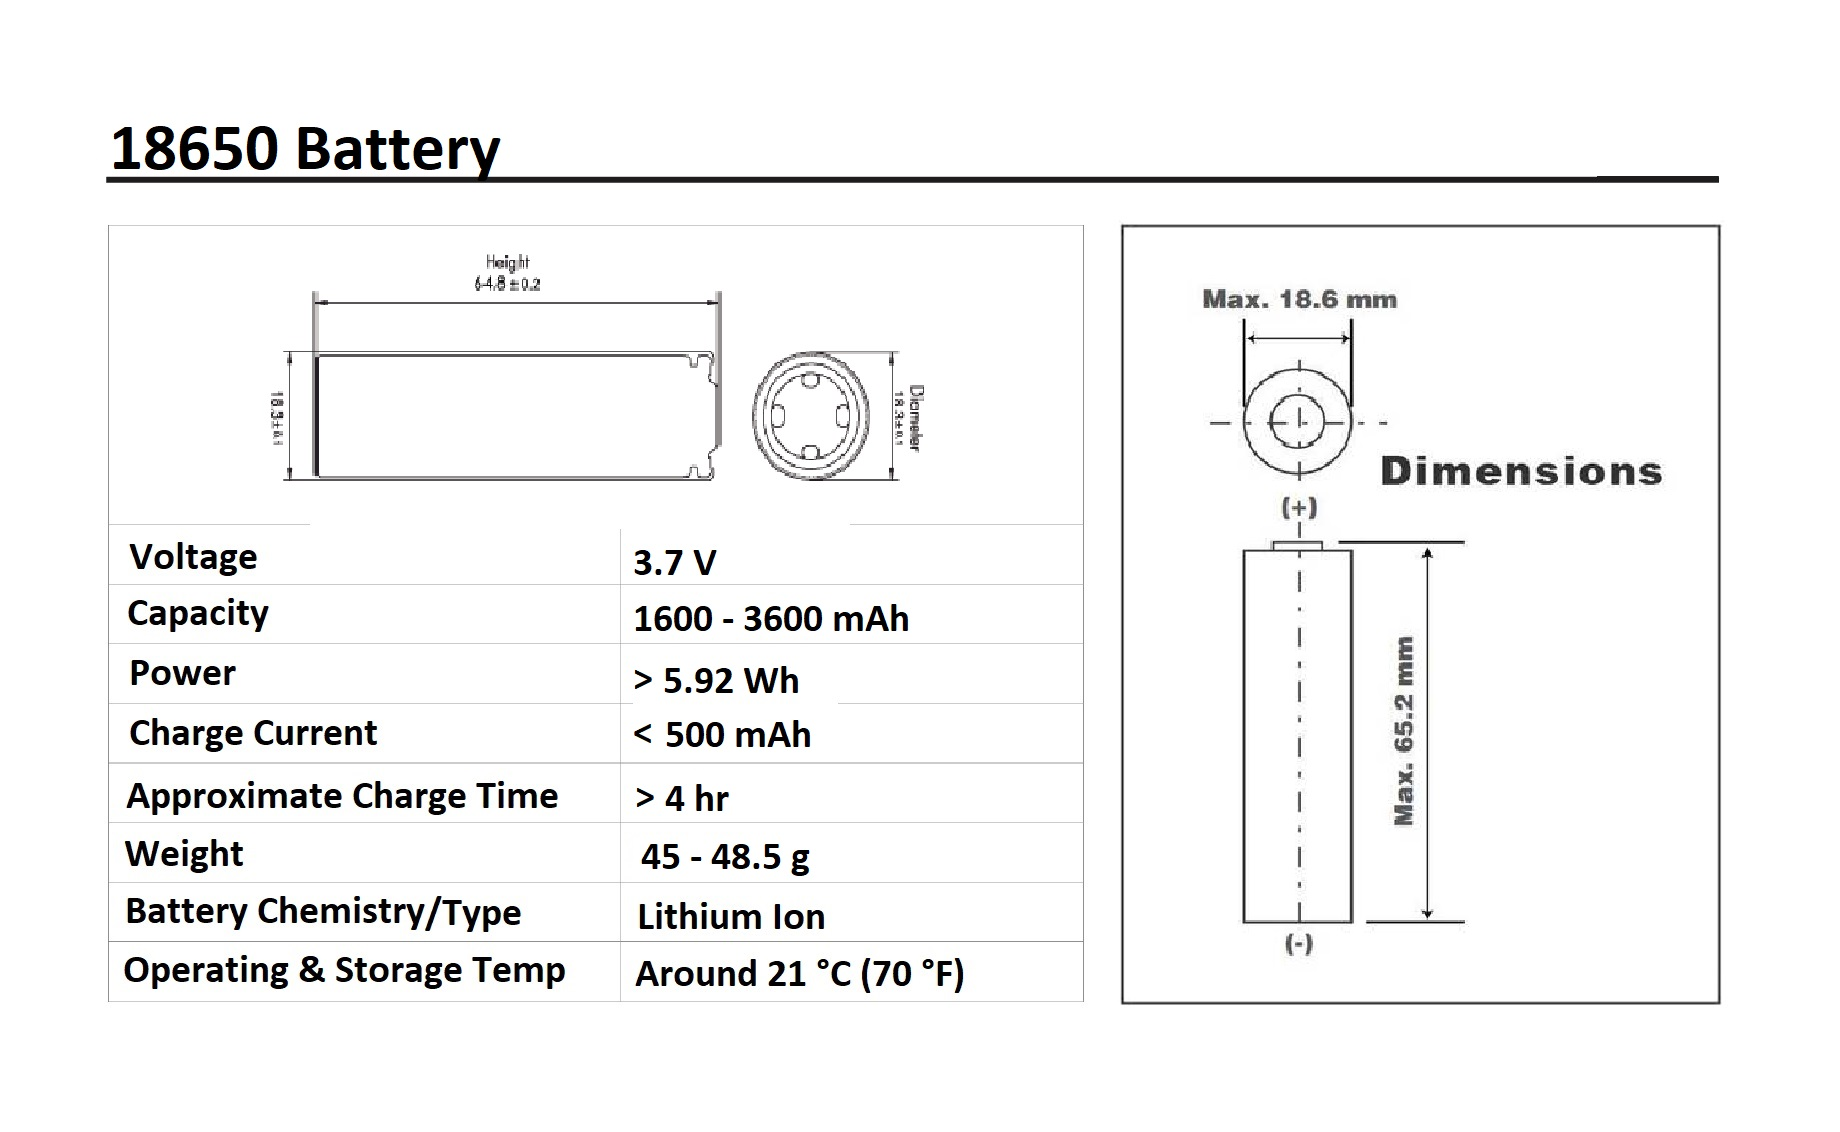
\includegraphics[width = 140mm, height = 80mm]{assets/18650_Battery.jpg}
				\caption{18650 Lithium Ion Battery Design Specification \label{overflow}}
			\end{figure}
		
		\subsection{LED Design Specification}
		LED specifications and 2 potential solutions detailed below.
			\begin{figure}[!htb]
				\centering
				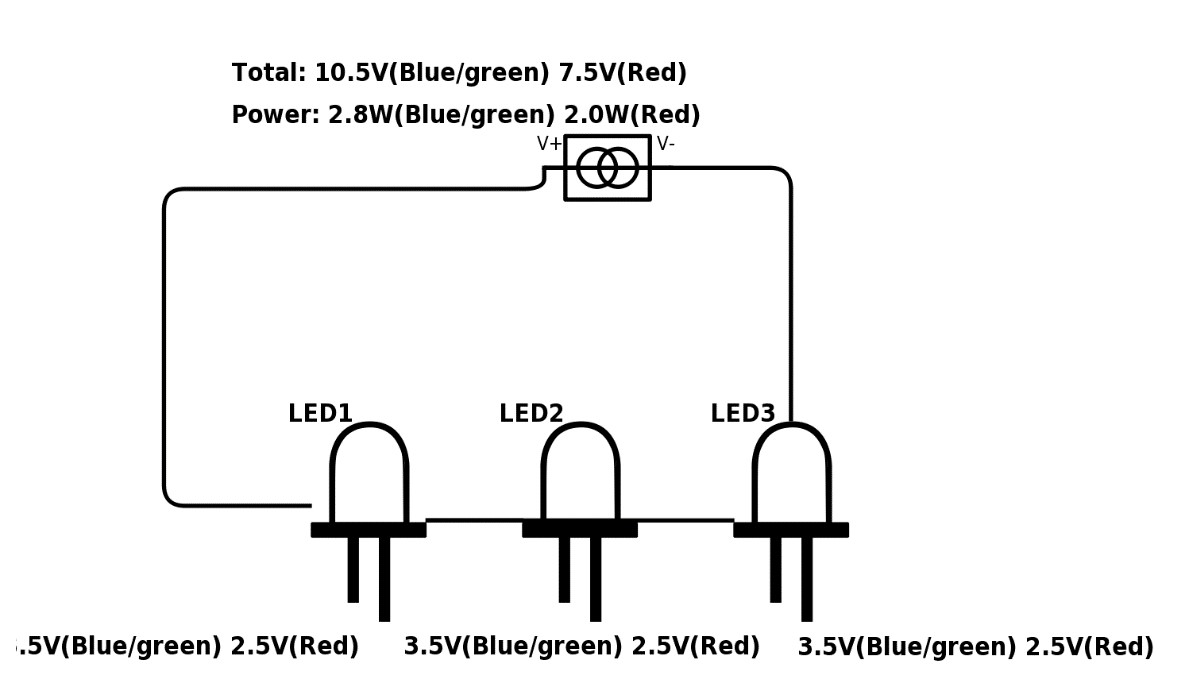
\includegraphics[height = 80mm]{assets/SeriesLED.jpg}
				\caption{Circuit diagram with LEDs in series \label{overflow}}
			\end{figure}
		
			\begin{figure}[!htb]
				\centering
				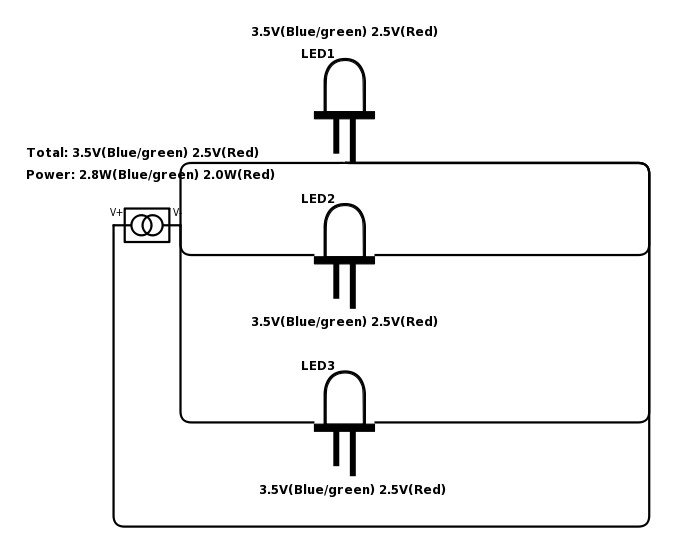
\includegraphics[height = 80mm]{assets/ParallelLED.jpg}
				\caption{Circuit diagram with LEDs in parallel \label{overflow}}
			\end{figure}
		
		\subsection{LED Specification Adjustments}
			The General Specifications have been adjusted to more accurately reflect the design choices and concept.		
			\begin{figure}[!htb]
				\centering
				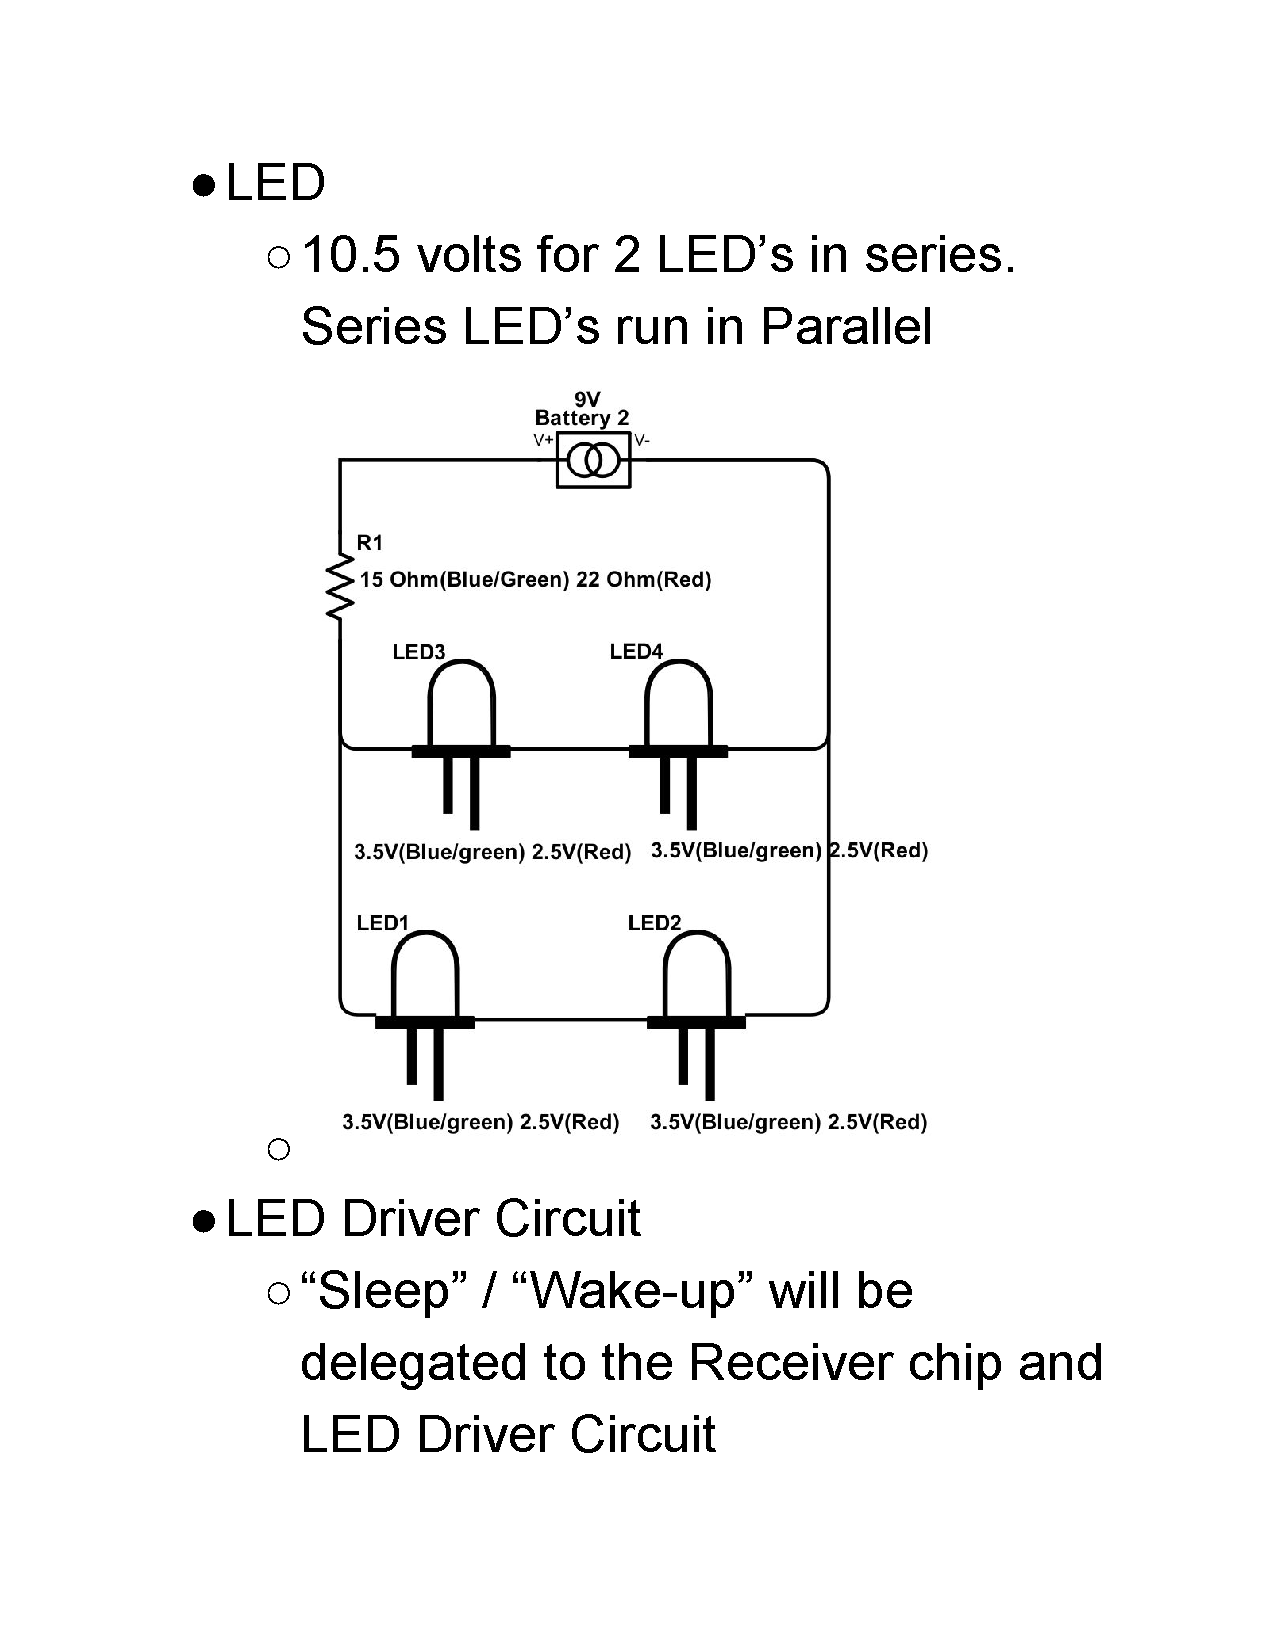
\includegraphics[width = 80mm, height = 90mm]{assets/3_General_Specifications.pdf}
				\caption{General Specification Adjustments \label{overflow}}
			\end{figure}
		
		\subsection{Wireless Design Specification}
			Specification of the wireless protocols at place, including the used 802.15.4 protocol
			\begin{figure}[!htb]
				\centering
				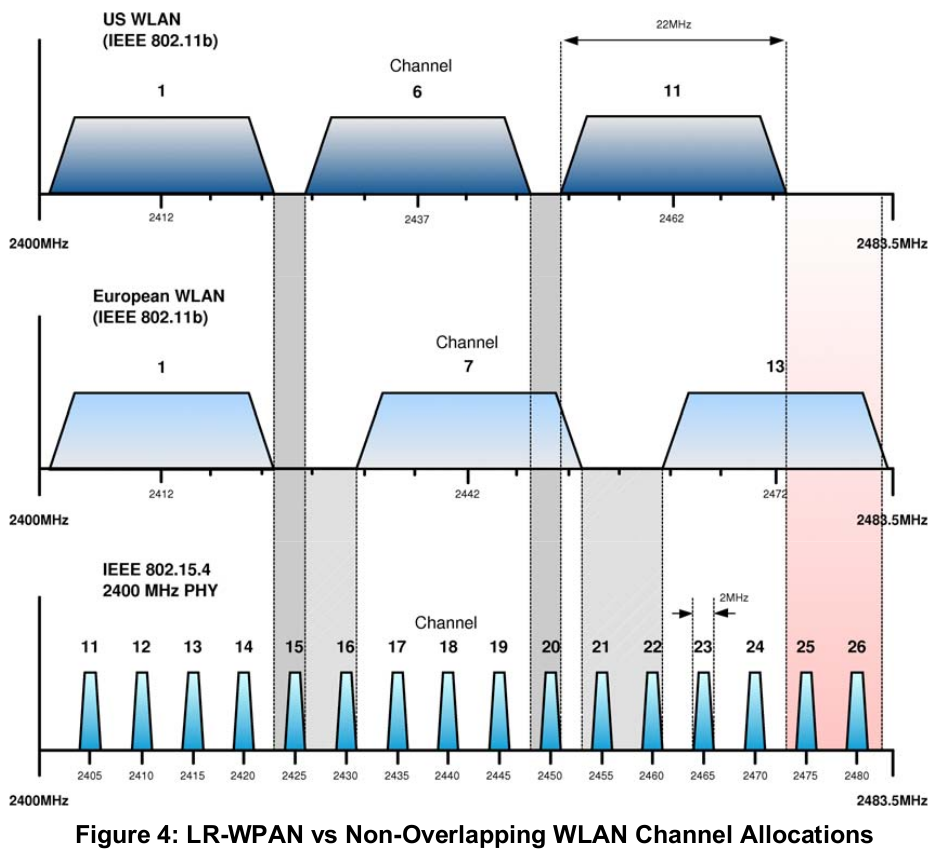
\includegraphics[height = 80mm]{assets/Zigbee.png}
				\caption{ \textbf{Zigbee Wireless Protocol} Uses Channels Above Wi-Fi \label{overflow}}
			\end{figure}
	
		\subsection{Gantt Chart}
			The Gantt Chart representing our intended and actual shedule is shown in the figure below
			\begin{figure}[ht!]
				\centering
				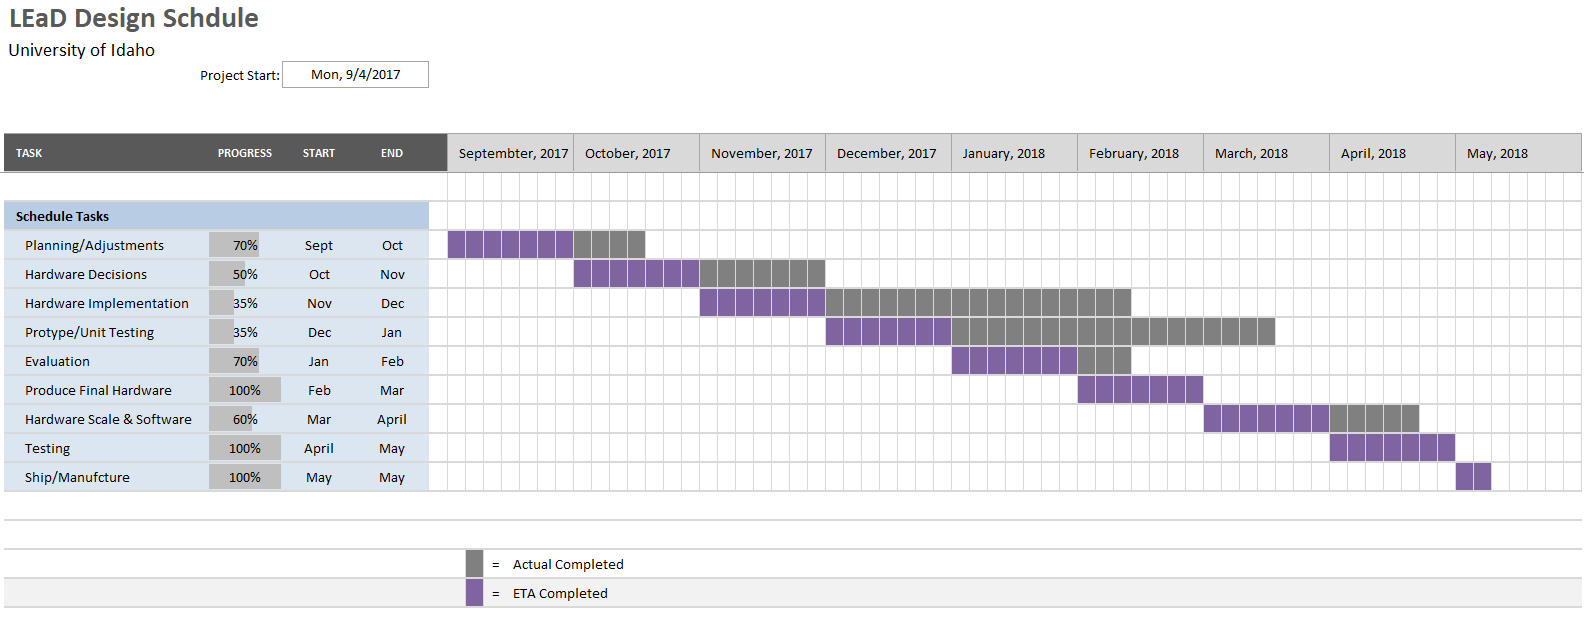
\includegraphics[width=170mm]{assets/Gantt_Chart_Shedule.png}
				\caption{Hardware List \label{overflow}}
			\end{figure}
		
		\subsection{Bill of Materials}
		The bill of materials (BOM) is shown below.
		
			\begin{figure}[ht!]
				\centering
				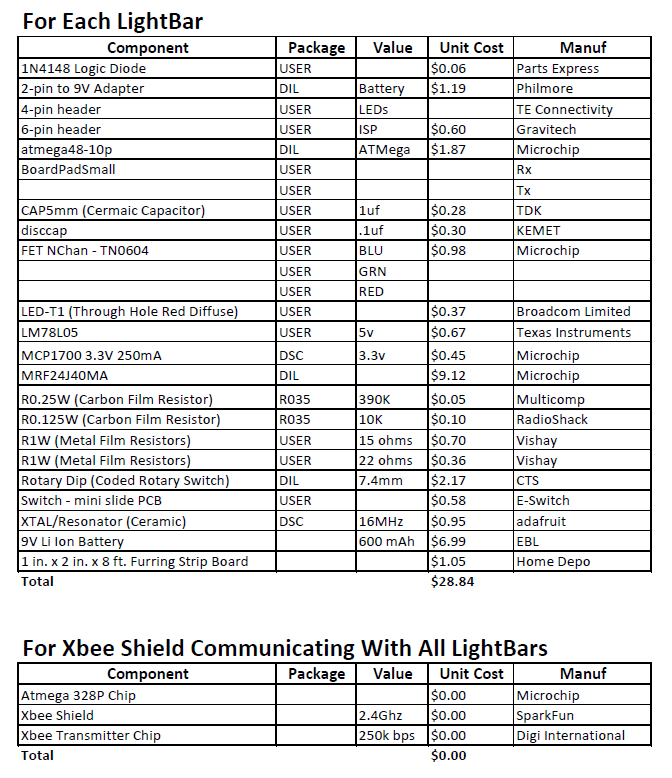
\includegraphics[width=170mm]{assets/Bill_of_Materials_Pg1.png}
				\caption{Bill of Matierals}
			\end{figure}
			
			\begin{figure}[ht!]
				\centering
				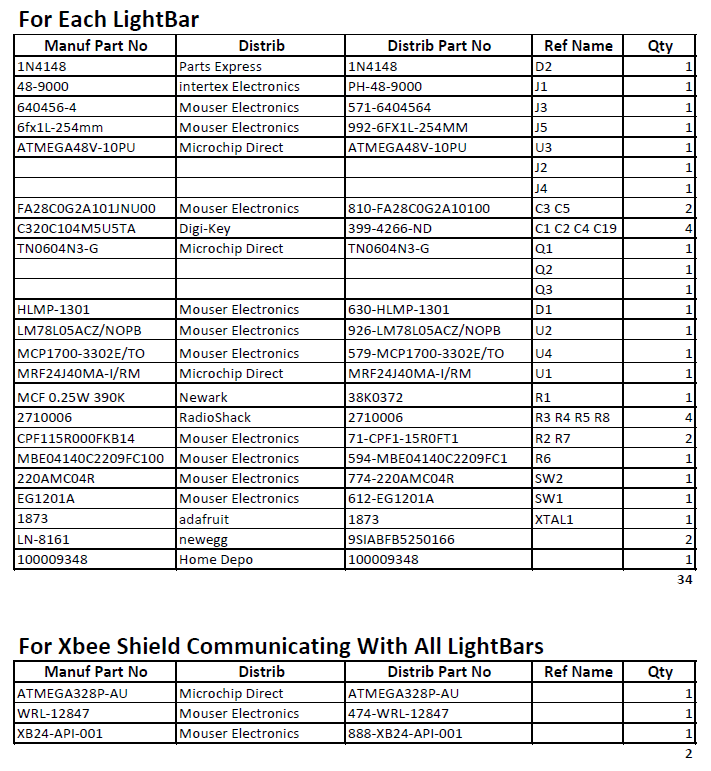
\includegraphics[width=170mm]{assets/Bill_of_Materials_Pg2.png}
				\caption{Bill of Matierals}
			\end{figure}
		
		\subsection{Prototype Progress}
			We have completed our first Wireless Lightbar prototype, utilizing 4 LEDs. The prototype can be viewed below:
			
			\begin{figure}[ht!]
				\centering
				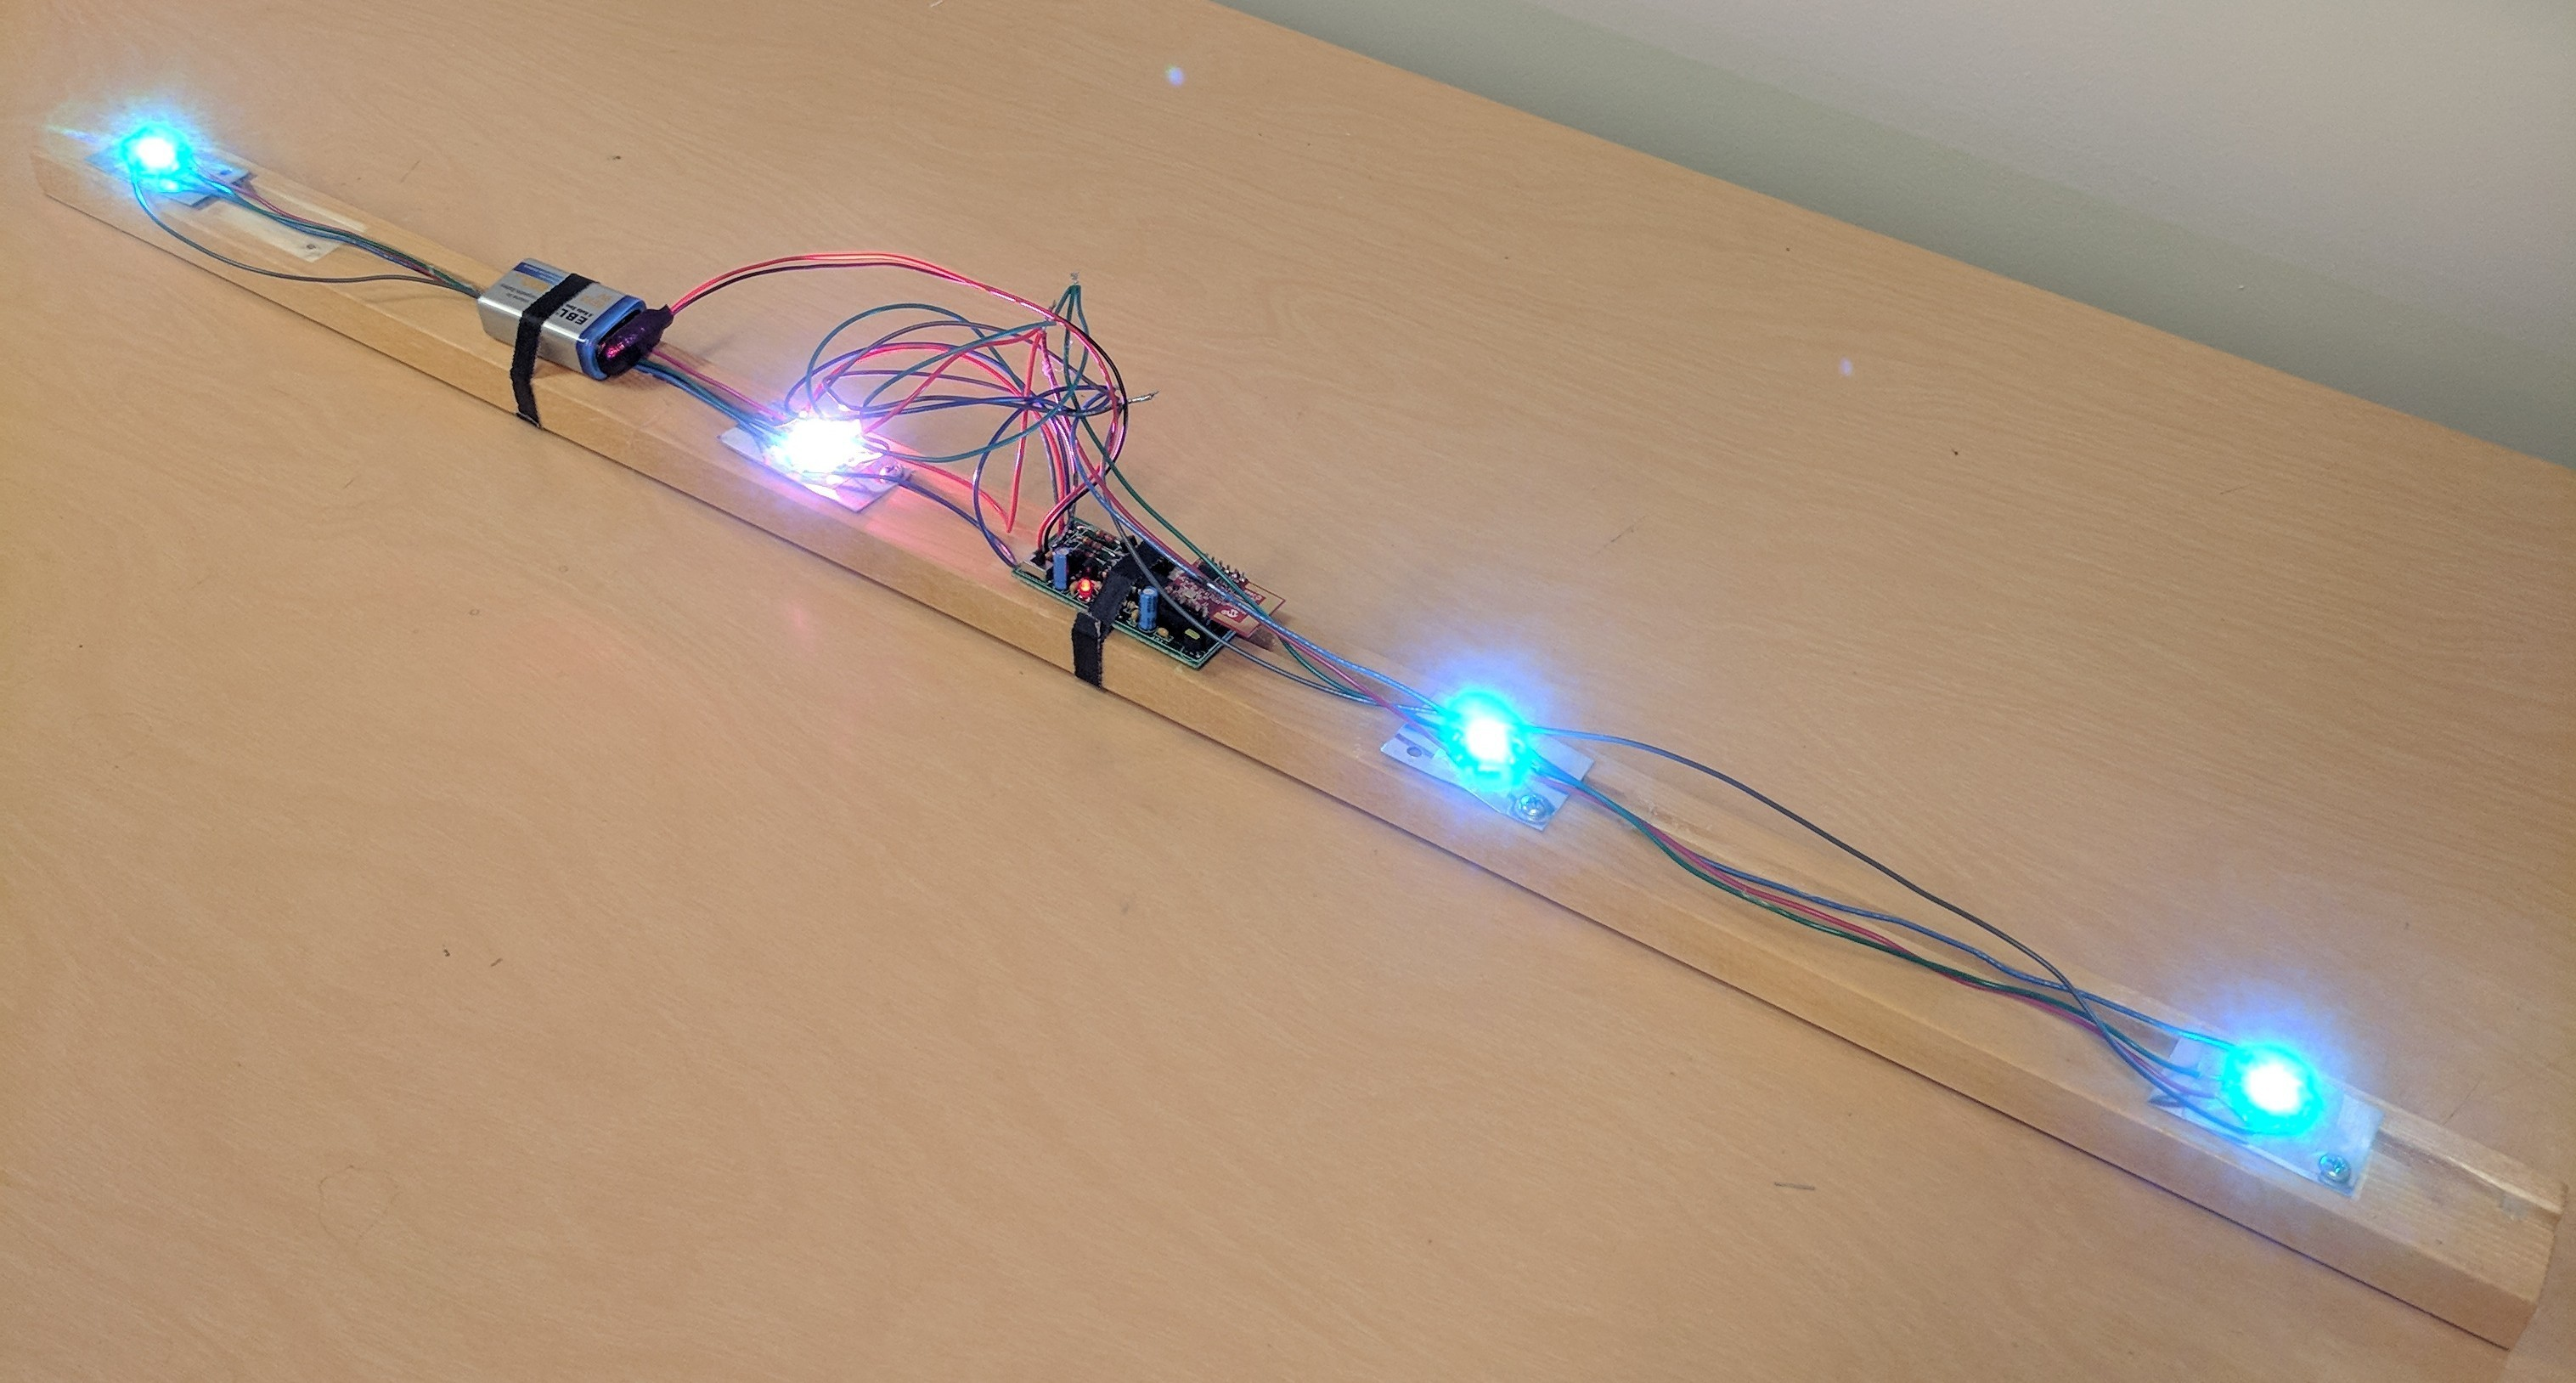
\includegraphics[width=70mm]{assets/prototype.jpg}
				\caption{Prototype One}
			\end{figure}
	
		\subsection{Hardware List/Cost of Materials}
			The figure below is the current Hardware list.
			
			\begin{figure}[ht!]
				\centering
				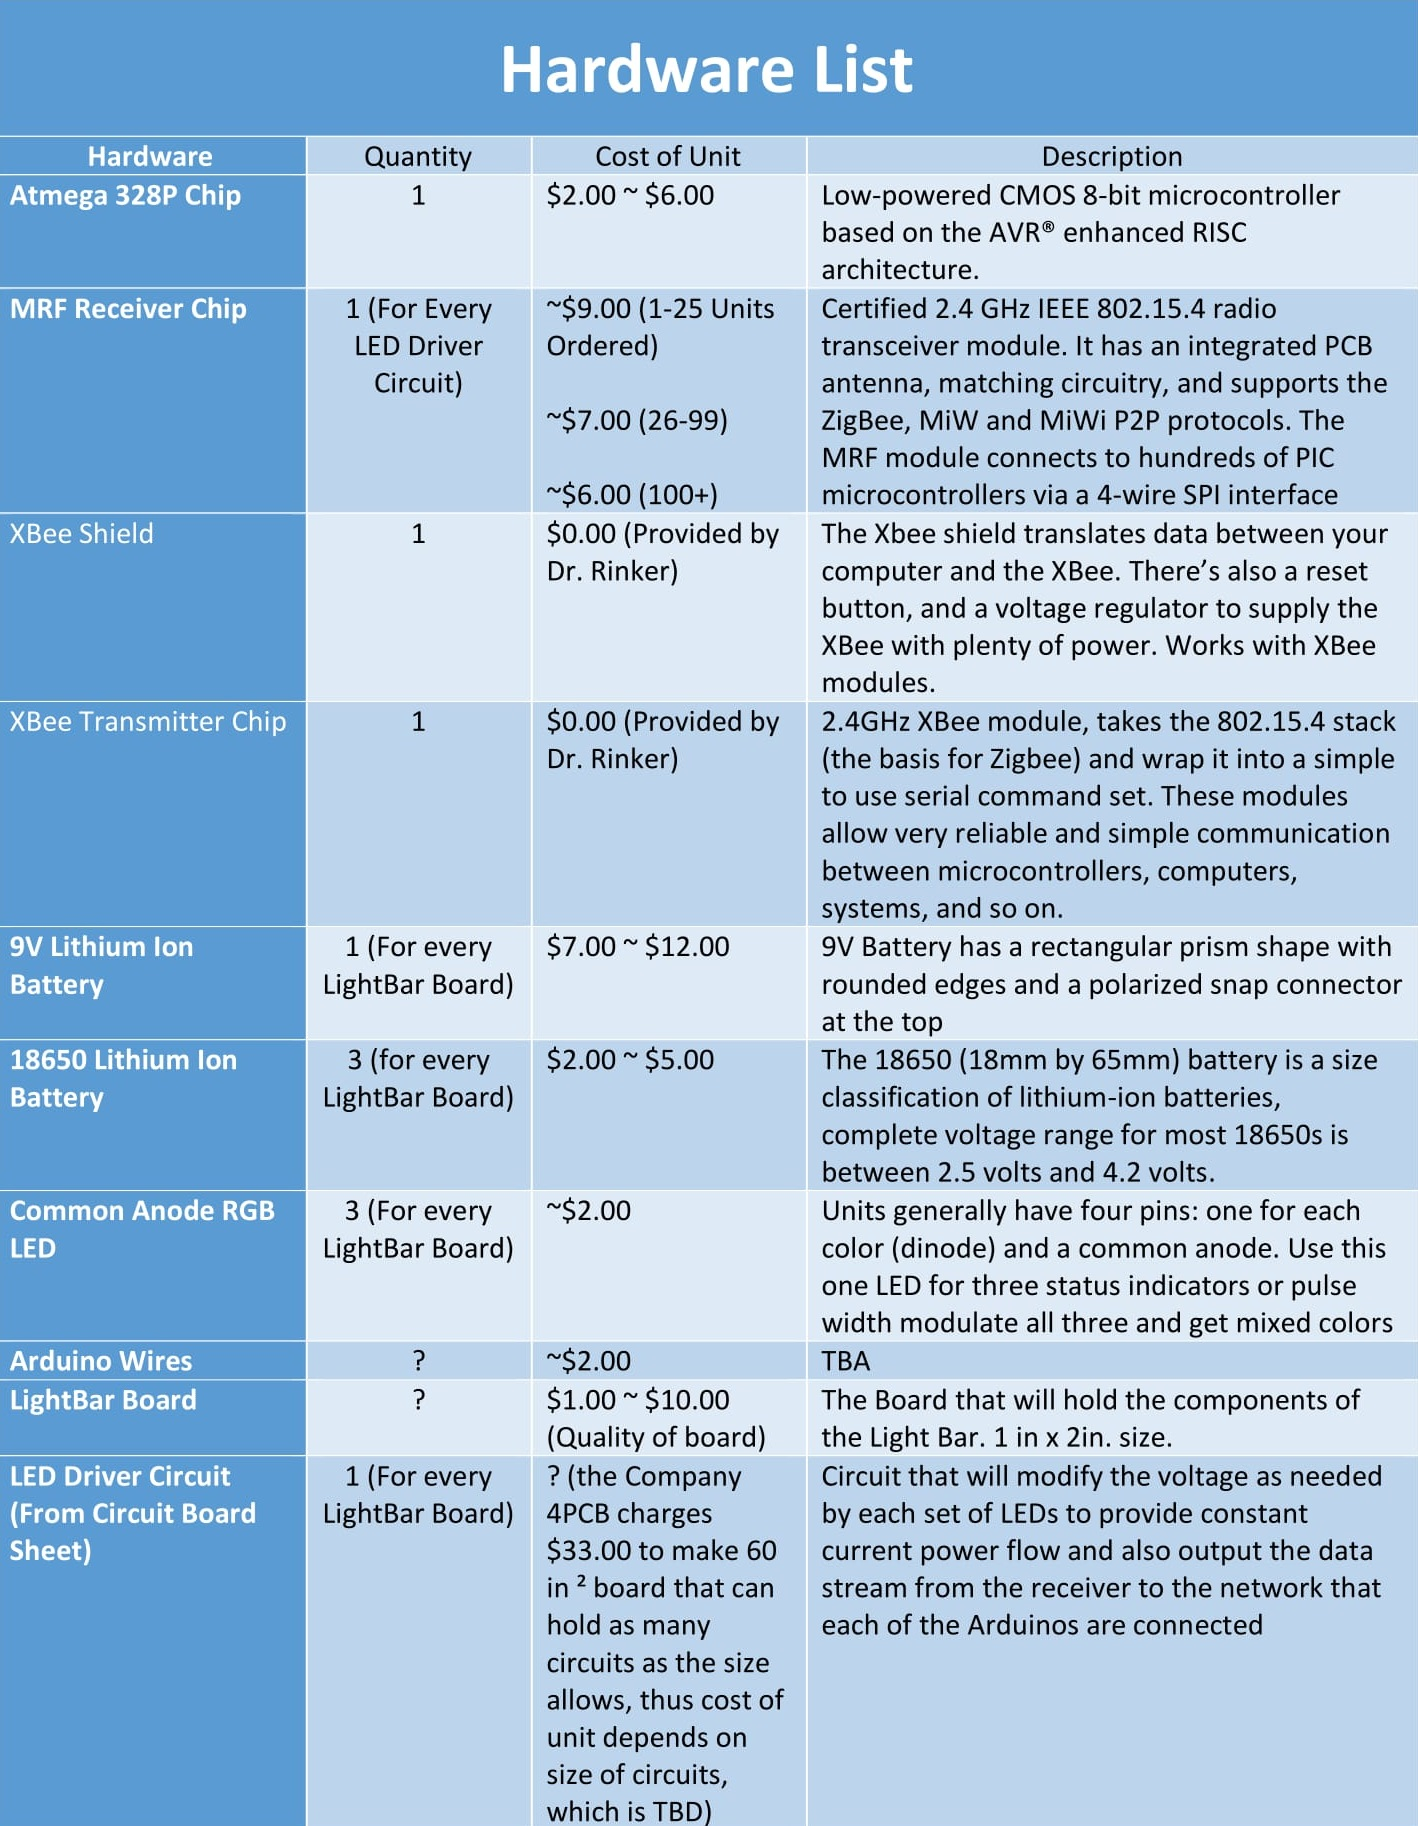
\includegraphics[width=110mm]{assets/HardwareList.jpg}
				\caption{Hardware List \label{overflow}}
			\end{figure}
		
		\clearpage
	
	\section{Computer Programs}
	NA-Too Long!
	
	\newpage
	
	\section{Vendor Data Sheets}
	
		\subsection{Xbee Transmitter Data Sheet}
			\begin{figure}[ht!]
				\centering
				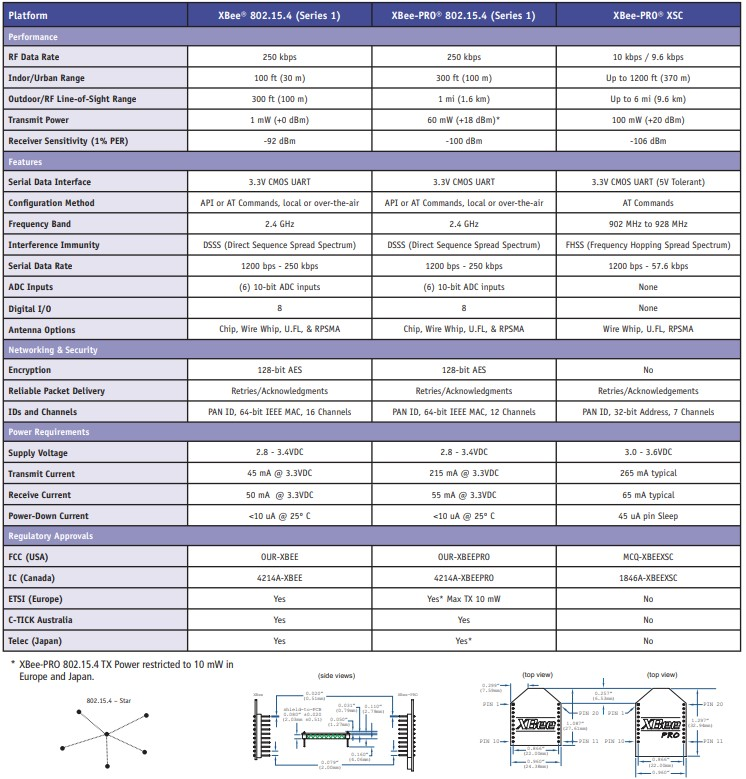
\includegraphics[height=175mm]{assets/Xbee_DataSheet.jpg}
				\caption{Xbee Transmitter Data Sheet \label{overflow}}
			\end{figure}
		
		\subsection{Atmega 328P Data Sheet}
			\begin{figure}[ht!]
				\centering
				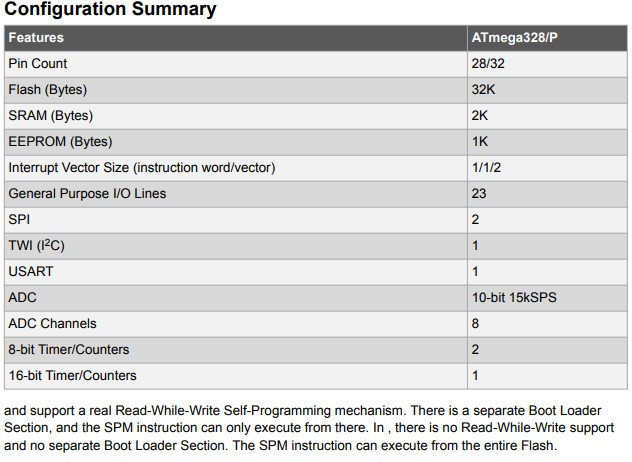
\includegraphics[width=125mm]{assets/Atmega_DataSheet.jpg}
				\caption{Atmega 328P Data Sheet Pg.1\label{overflow}}
			\end{figure}
		
			\begin{figure}[ht!]
				\centering
				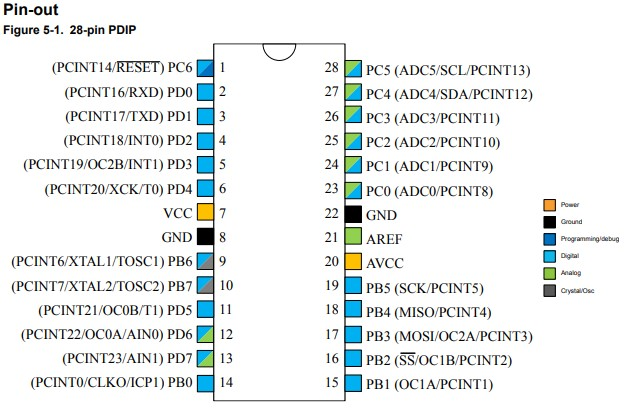
\includegraphics[width=125mm]{assets/Atmega_DataSheet2.jpg}
				\caption{Atmega 328P Data Sheet Pg.2\label{overflow}}
			\end{figure}
			
			\clearpage
			
		\subsection{Xbee Shield Data Sheet}
			\begin{figure}[ht!]
				\centering
				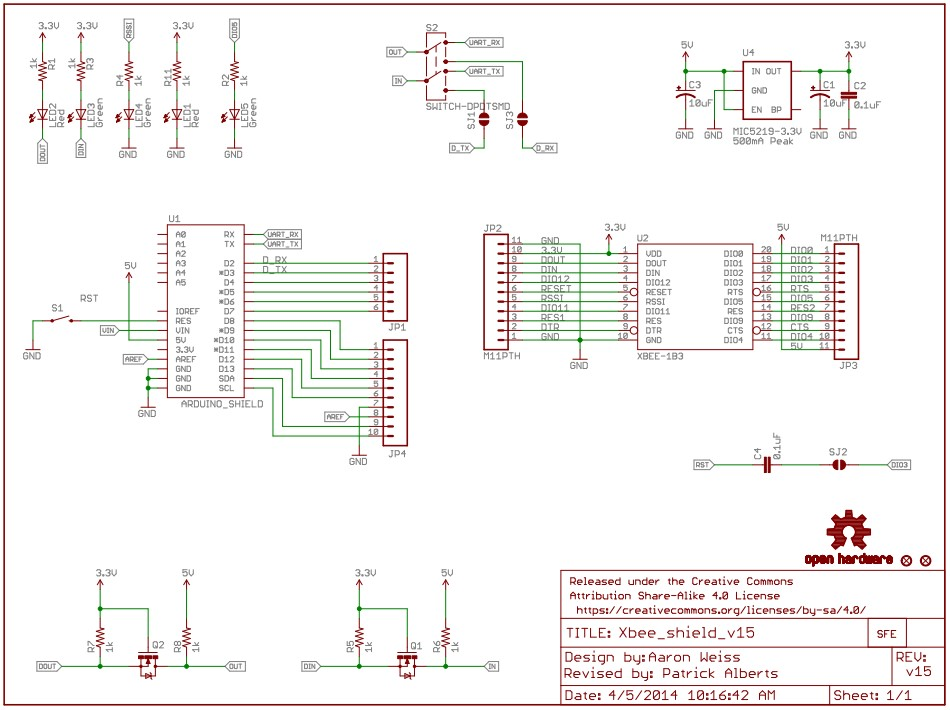
\includegraphics[height=130mm]{assets/Xbee_Shield_DataSheet.jpg}
				\caption{Xbee Shield Data Sheet \label{overflow}}
			\end{figure}
		
			\clearpage
		
		\subsection{9V Battery Data Sheet}
			\begin{figure}[ht!]
				\centering
				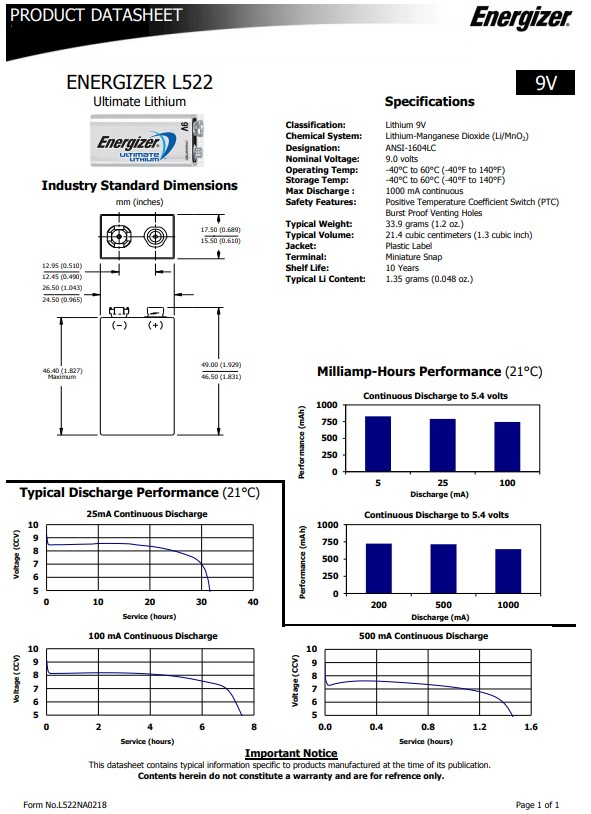
\includegraphics[height=200mm]{assets/9V_Battery_DataSheet.jpg}
				\caption{9V Battery Data Sheet \label{overflow}}
			\end{figure}
	
	\clearpage
	
	\section{Shedule}
	
		\subsection{Timeline - Diagram}
		This is the most recent timeline for the Wireless Tower of Lights project\\
		{ \setstretch{2.0}		
			\scalebox{1}{  		
				\begin{tabular}{r |@{\tline} l}  			
					September  & Planning/Adjustments/Finalize Program Flow         \\			
					October & Hardware Decision/Hardware Tinkering (Arduino/Xbee)            \\			
					November & Hardware Implementation and Initial Prototyping\\			
					December & Prototype Product/Unit Testing     \\			
					January & Product Improvement, Evaluation, and Final Product Hardware Decisions \\			
					February & Implementing and Producing Final Hardware\\			
					March  & Hardware Scale Testing, Software Improvements\\			
					April  & Testing       \\			
					May & Ship/Manufacture (Deliver product)         \\			
				\end{tabular}  		
			}  	
		}
	
		\subsection{Schedule - Orignally Planned}
			This is the original schedule, as planned by the LEaD Design Team
			\begin{figure}[ht!]
				\centering
				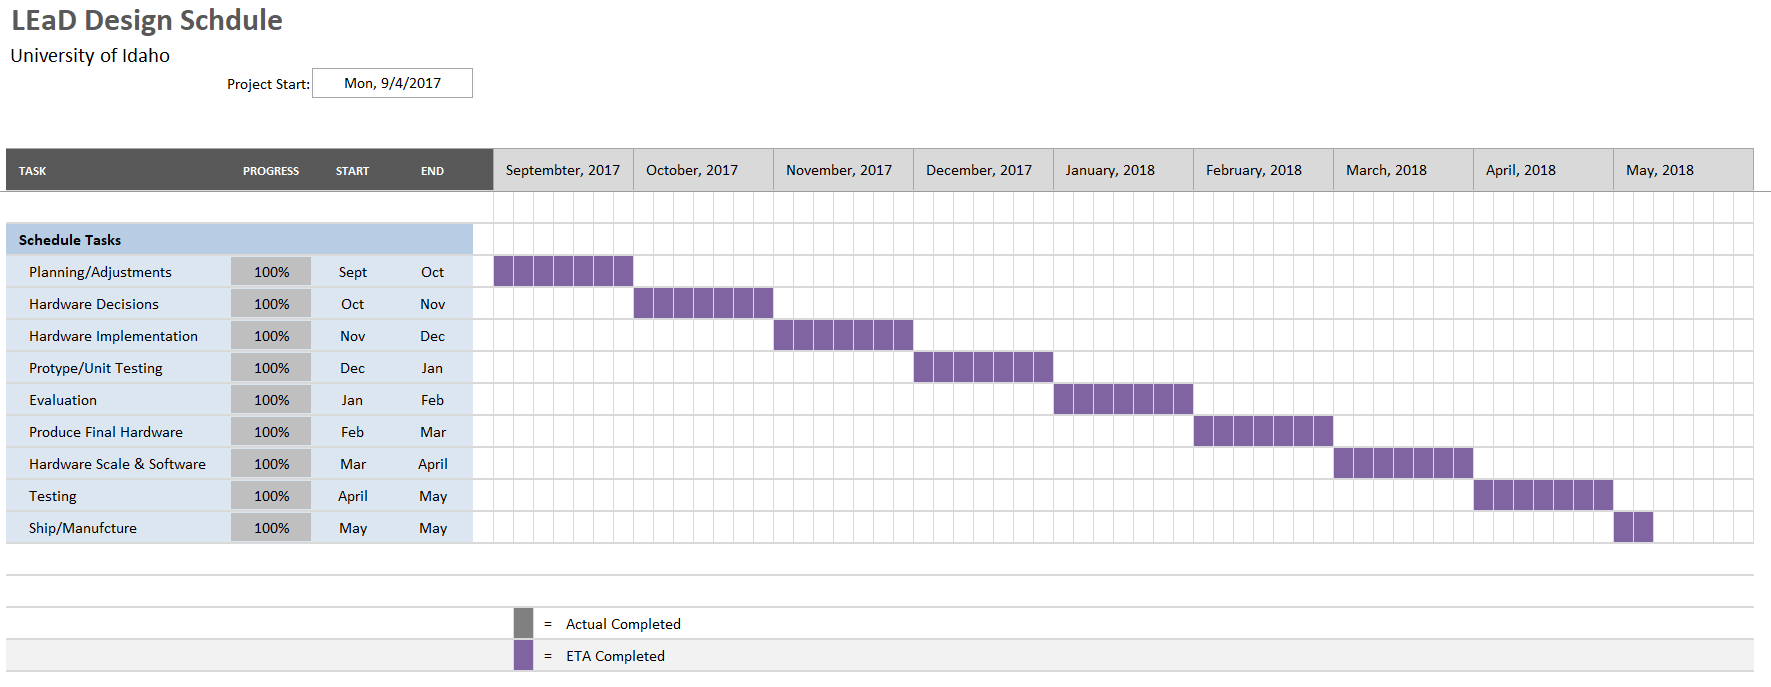
\includegraphics[width = 180mm, height = 100mm]{assets/Gantt_Chart_Shedule_Planned.png}
				\caption{Schedule - Orignally Planned \label{overflow}}
			\end{figure}
		
		\subsection{Schedule - Executed}
			This is the executed schedule, as accomplished by the LEaD Design Team
			\begin{figure}[ht!]
				\centering
				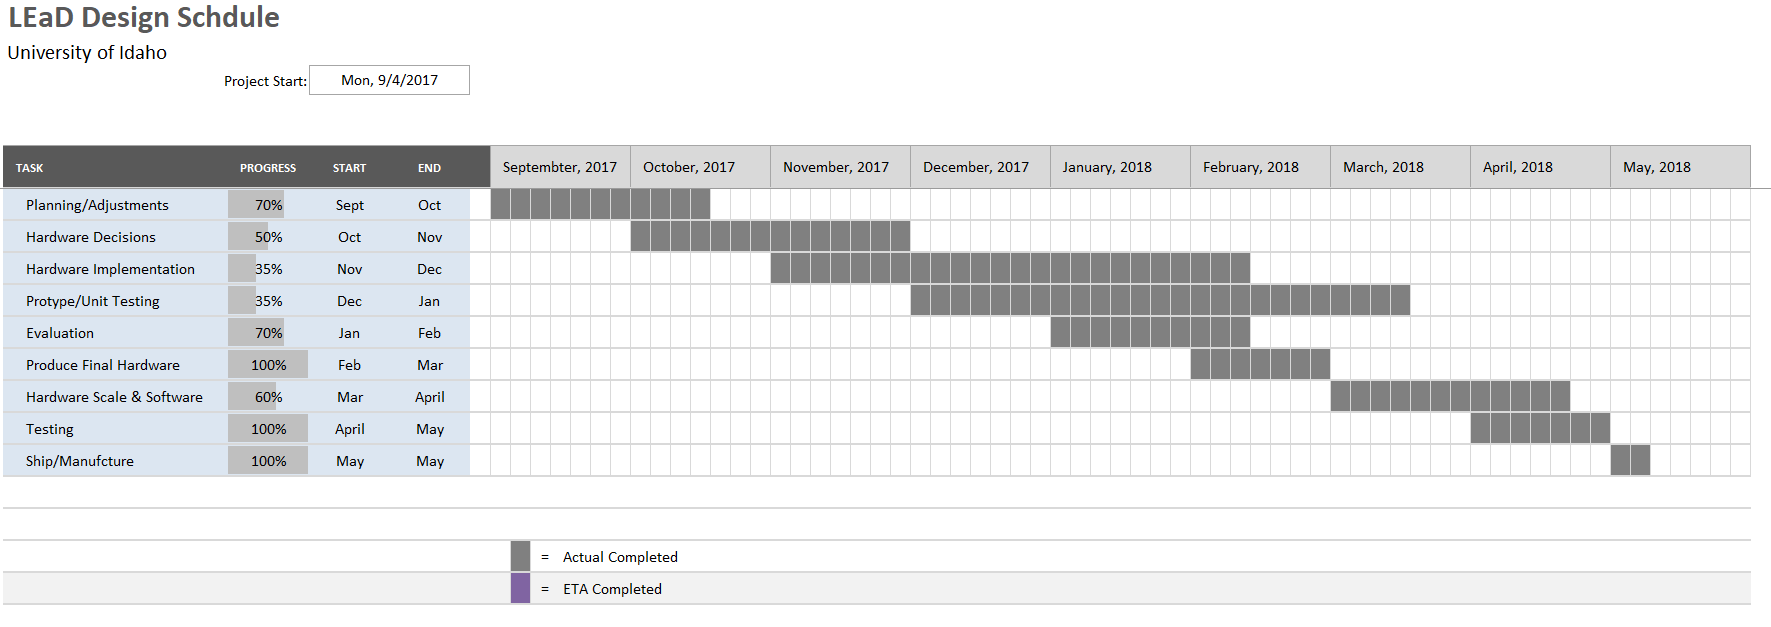
\includegraphics[width = 180mm, height = 100mm]{assets/Gantt_Chart_Shedule_Executed.png}
				\caption{Schedule - Executed \label{overflow}}
			\end{figure}
		
		\clearpage
		
	\section{DFMEA Worksheet}
		The DFMEA is shown on the following page.
		
		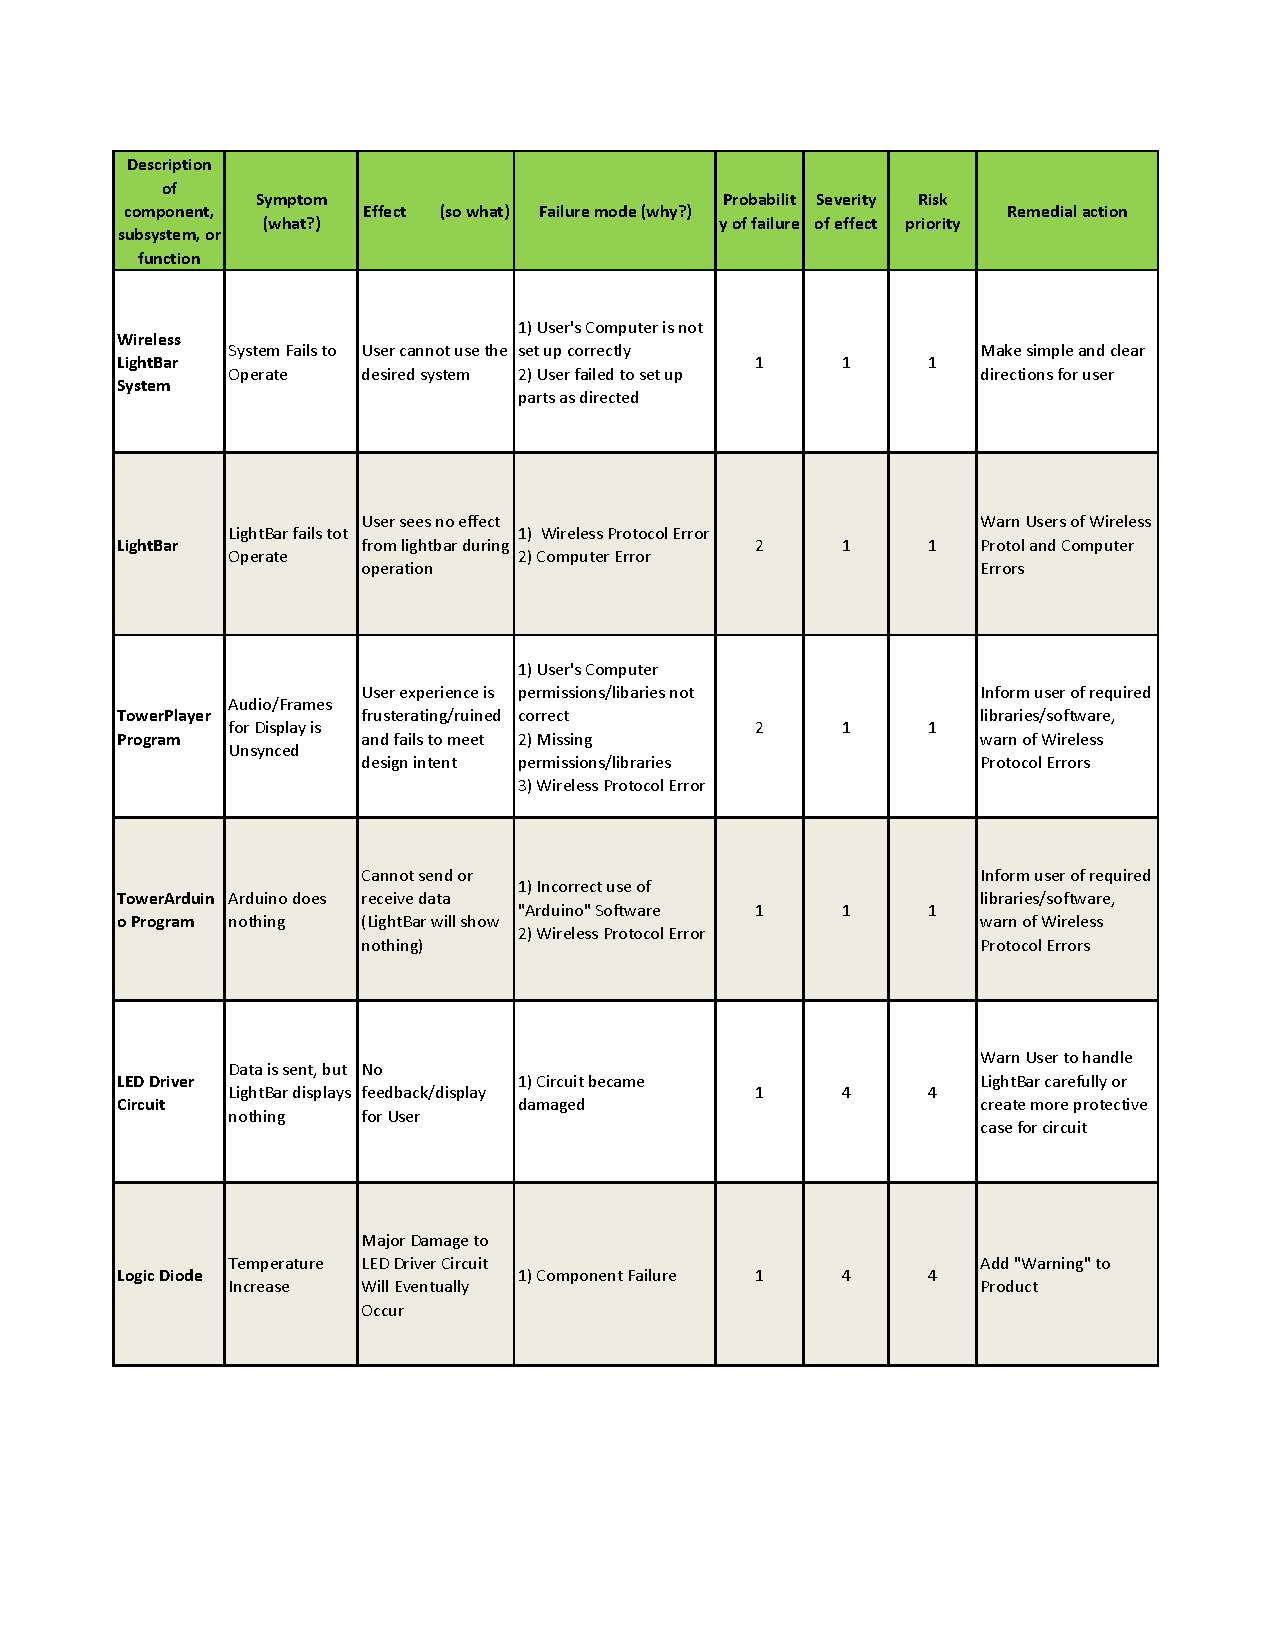
\includepdf[pages={-}, scale = 1, pagecommand={\null\vfill\captionof{figure}{DFMEA}}]{assets/DFMEA_LEaD_Design_PDF.pdf}
		
		\newpage
		
	\section{Overview of Folder/File Organization}
	NA

\end{document}
